\chapter{Implementation, Result, and Analysis}
\section{Overview of the approach}
Before training, we have reviewed what the chosen network requires as input.
Since we are training using synthetic dataset that would imitate our target
scenarios, we focused on generating diverse and representative samples.
\section{Dataset Preparation \& Preprocessing}
The network expects:
\begin{itemize}
    \item \textbf{Two images:} the reference image, and the target image. Stored as numpy arrays.
    \item \textbf{Two sets of keypoints:}
          \begin{itemize}
              \item \textbf{Reference keypoints:} An array of keypoint coordinates found in the reference
                    image. It has a shape of $(N, 2)$, where N is the number of keypoints, and the coordinates are (x, y).
              \item \textbf{Target keypoints:} An array of keypoint coordinates found in the target image that correspond to the reference keypoints. It has the same shape $(N, 2)$.
          \end{itemize}
    \item \textbf{Matches:} An array of shape $(N, 2)$ that stores the indices of the matching keypoints. For example, $[i, j]$ means that the i-th keypoint in the reference keypoints matches the j-th keypoint in the target keypoints.
    \item \textbf{Homography Matrix: } A 3 by 3 matrix that relates the reference icon to the target one. It is used to transform points from the reference to the target image, and vice versa.
    \item \textbf{Two binary masks:} Binary masks of the target image that indicates the region where the pixel exists. This is useful to separate the foreground from the background.
\end{itemize}
These elements would be stored as a zipped numpy file (.npz) to be later accessed during training and evaluation, and stored in a folder structure that mirrors the dataset organization.
\subsection{Data Synthesis}
\subsubsection{General Approach}
To create a diverse and representative dataset, we employed data synthesis
techniques that will allow us to experiment with various scenarios. Our general
idea consists of cropping a region of interest from the selected gaming frames,
this will help us simulate different viewpoints where the targeted 2D template
may appear.
\begin{figure}[H]
    \centering
    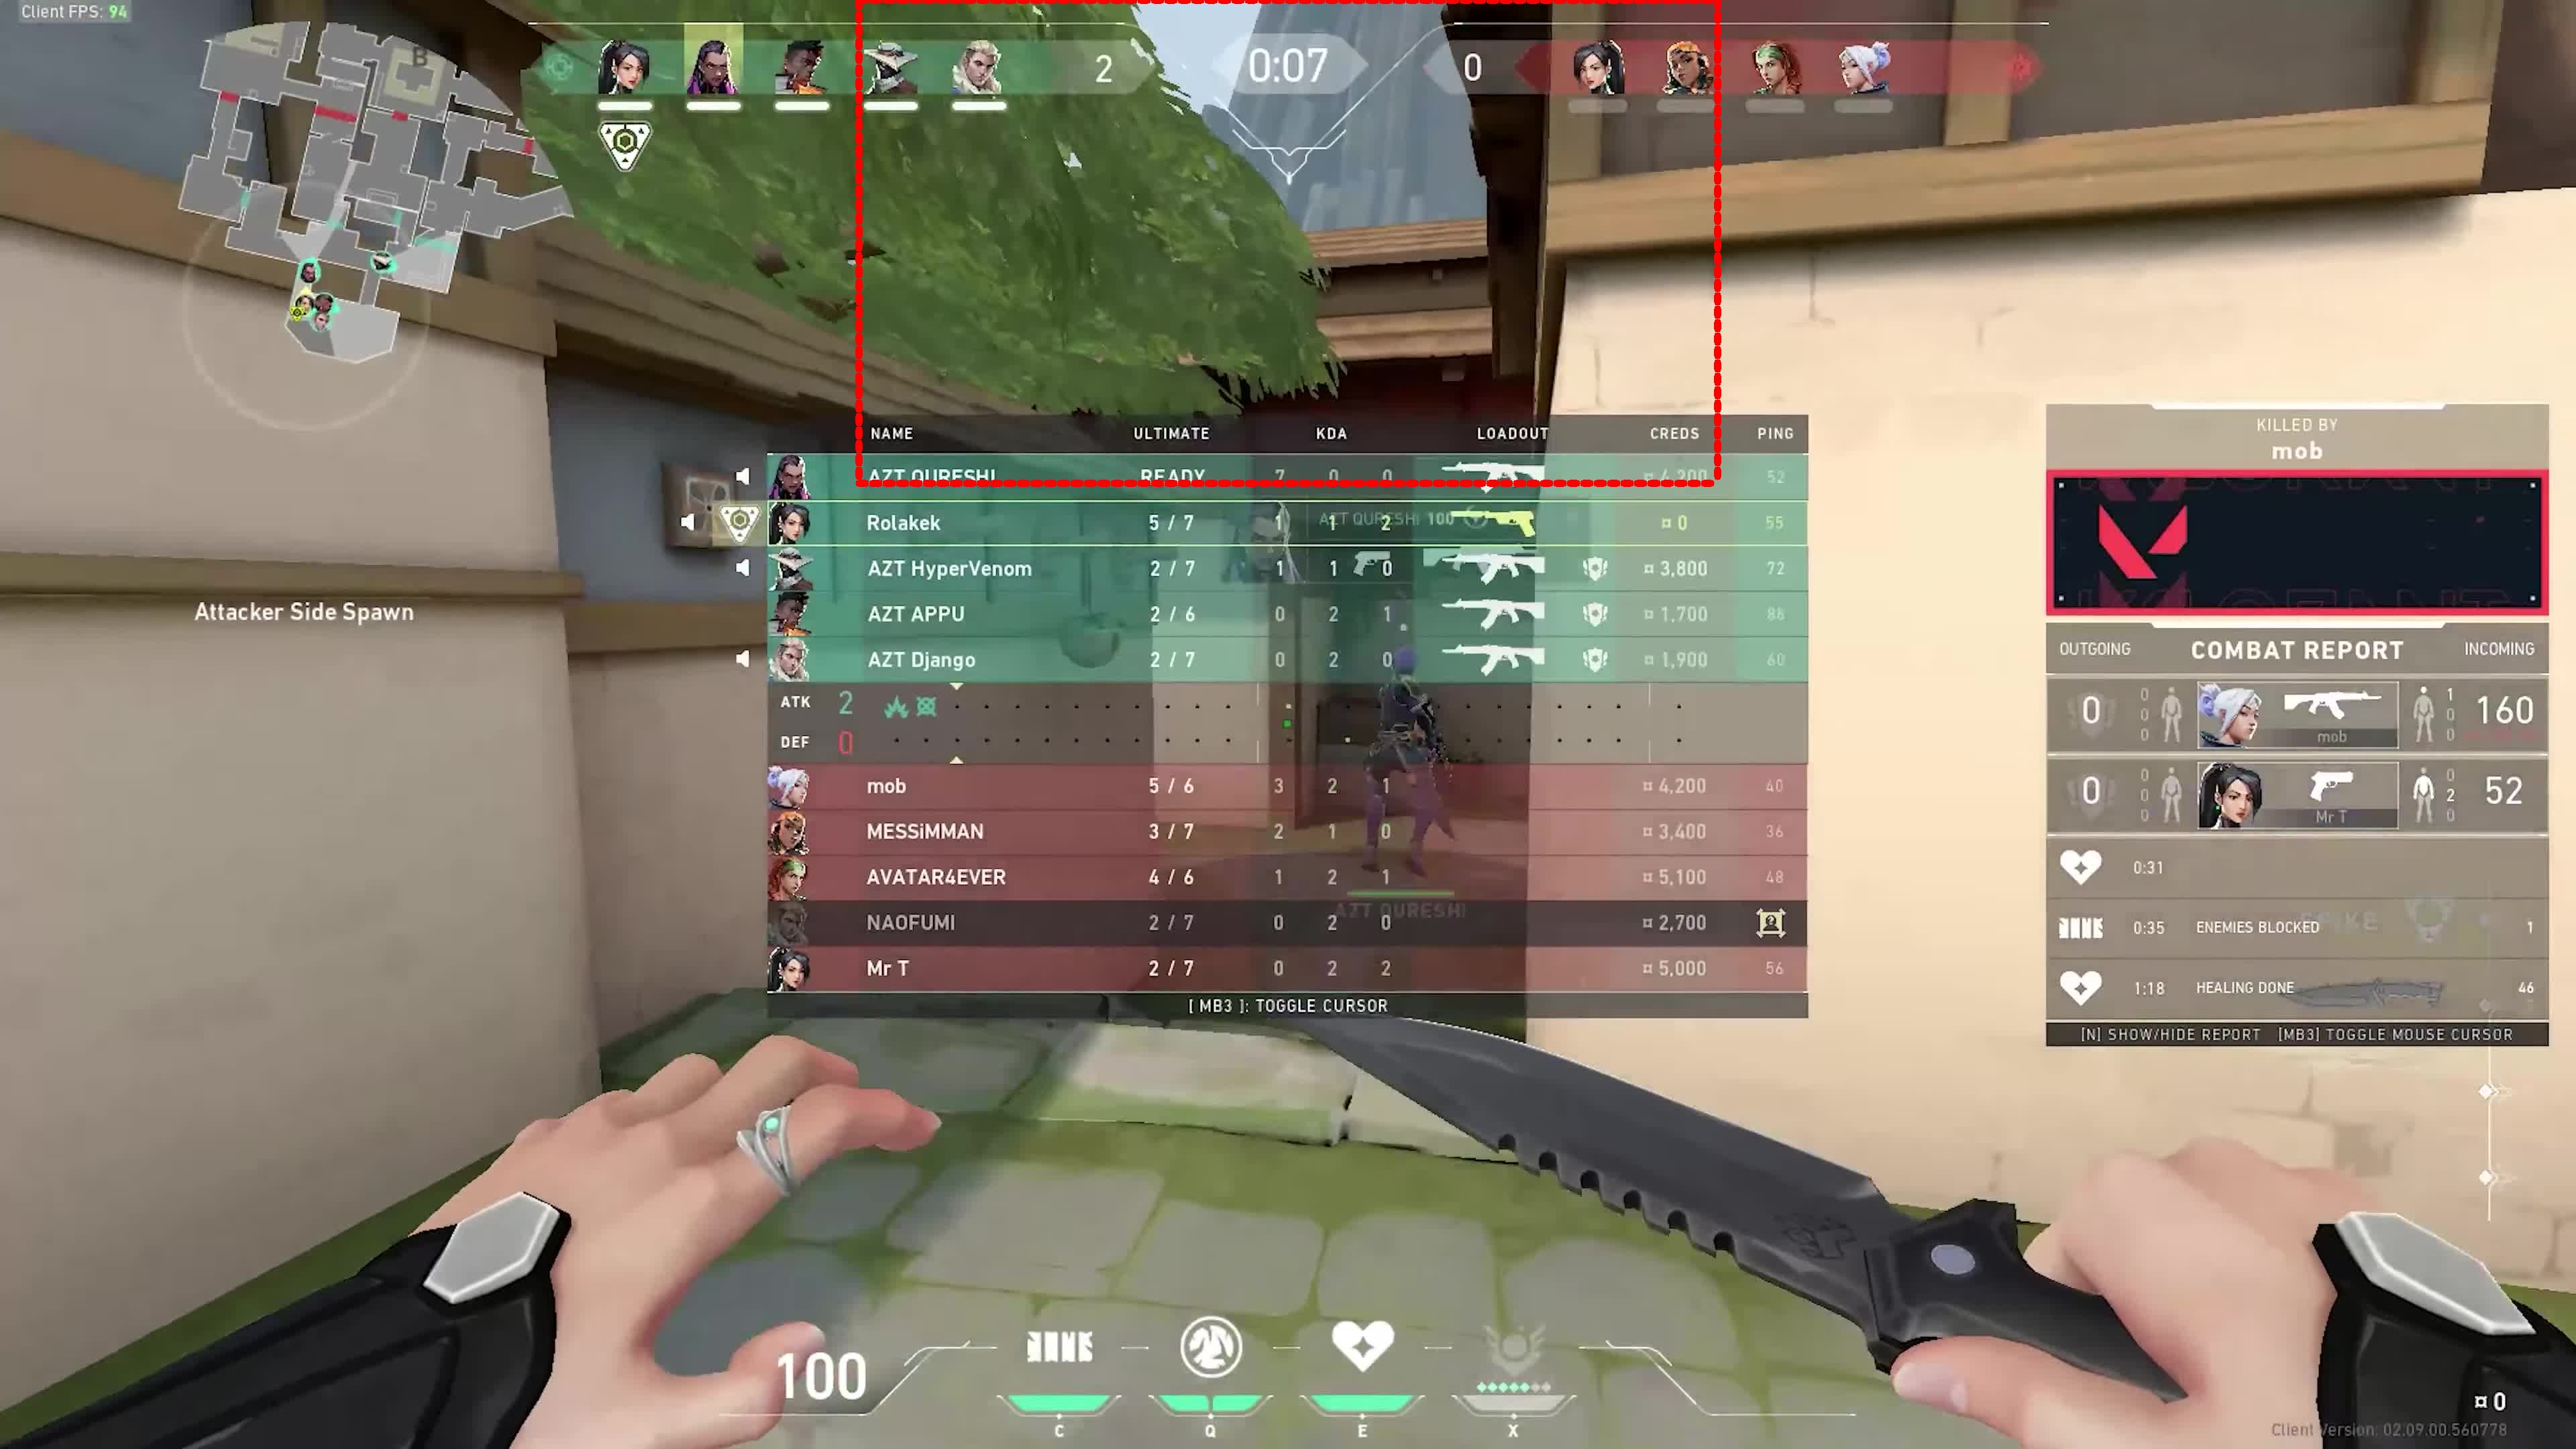
\includegraphics[width=\textwidth]{ressources/roi.jpg}
    \caption{Example of a cropped region of interest from a gaming frame.}
    \label{fig:roi_example}
\end{figure}
This newly selected area will serve as our background for the rest of the synthesis process. Then, we select an icon from our set of templates, which will be our target during training. We overlay our icon onto the background at the center, and we ensure that the icon is fully contained within the background region by downscaling it slightly and continuously till it fits perfectly.
\begin{figure}[H]
    \centering
    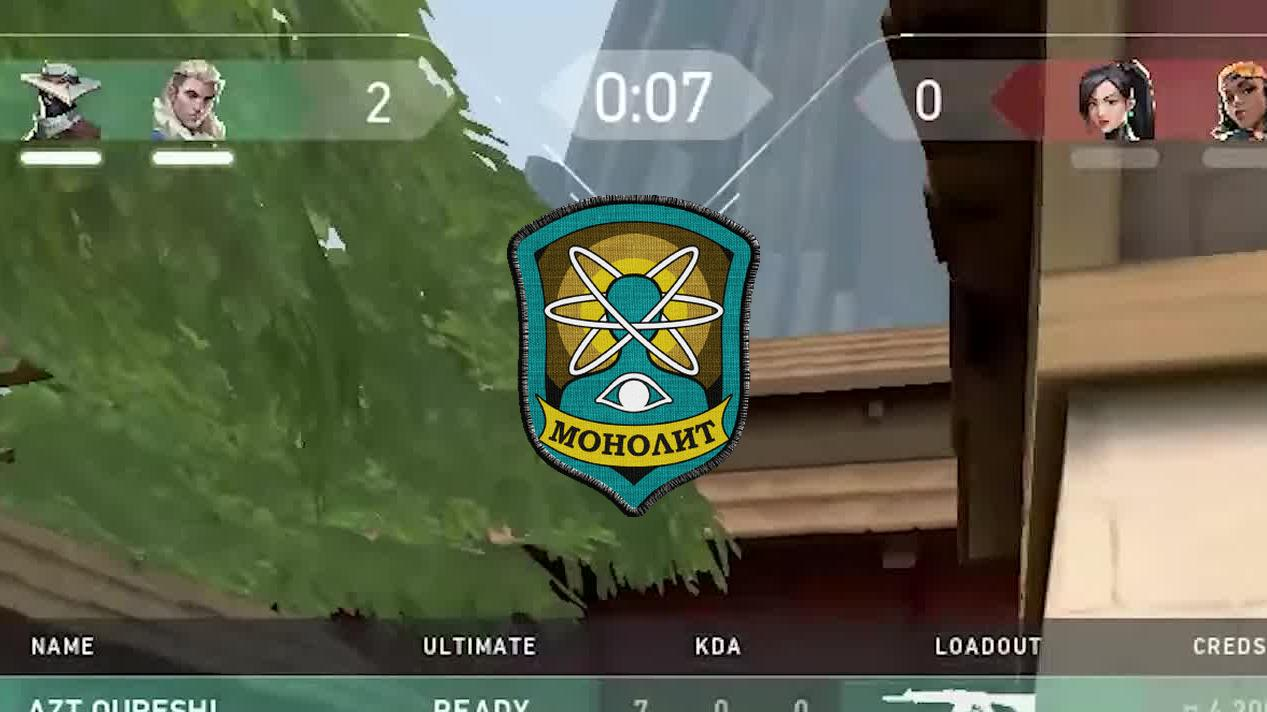
\includegraphics[width=0.9\textwidth]{ressources/image1.jpg}
    \caption{Example of the icon overlaid on the background.}
    \label{fig:overlay_example}
\end{figure}
While this describes our general design principle for synthetic data generation, the process was refined over several iterations to address specific challenges such as background complexity, icon transformations, and the robustness of extracted keypoints.
\begin{comment}
\begin{itemize}
    \item Scaling: We randomly scale the icon by a factor between 1.0 and 3.0
    \item Rotation: We randomly rotate the icon by an angle between -30 and 30 degrees.
    \item Translation: We randomly translate the icon by a few pixels in both x and y
          directions, while insuring that the icon remains within the bounds of the
          background.
    \item Color Jittering: We apply random changes to the brightness, contrast,
          saturation, and hue of the icon to create variations in appearance.
    \item Gaussian Noise: We add random Gaussian noise to the icon to simulate real-world
          noise.
\end{itemize}
\end{comment}

\section{Training Procedure \& Experimental Setup}
Our chosen approach consists of training the network on synthetic data using a
teacher-student framework. In the early stages, we kept the same teacher model
used by XFeat\cite{xfeat2023}. ALIKE, was used as a third party teacher tool to
extract ground truth keypoints from our training images.
\begin{figure}[H]
    \centering
    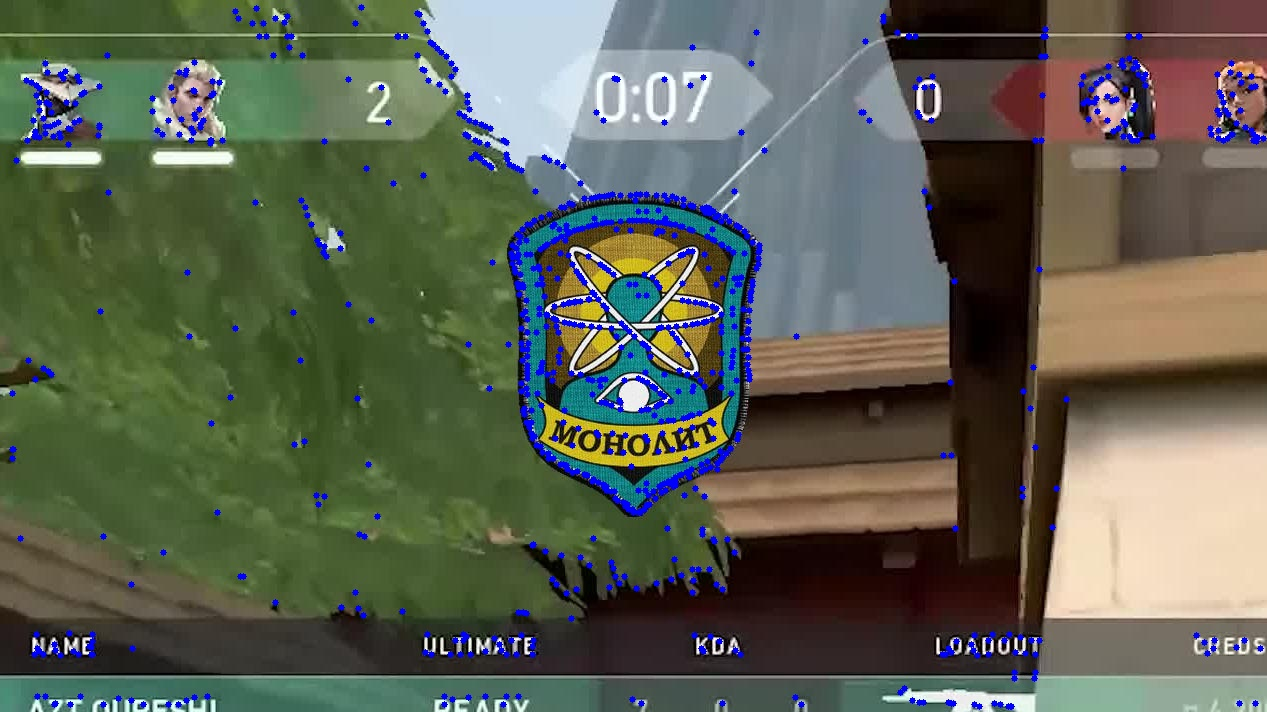
\includegraphics[width=0.8\textwidth]{ressources/image1_keypoints.jpg}
    \caption{Overview of extraction process.}
    \label{fig:teacher_student}
\end{figure}
We then generate a binary mask showing the presence of the icon within the background.
\begin{figure}[H]
    \centering
    
\includegraphics[width=0.8\textwidth]{ressources/mask_1.png}
    \caption{Example of the binary mask generated for the icon.}
    \label{fig:binary_mask}
\end{figure}
This mask is used to filter out keypoints that do not belong to the icon, ensuring that only relevant features are considered during training. This would teach the model to focus only the keypoints and data existing within the icon region , which is what we want to achieve.
\begin{figure}[H]
    \centering
    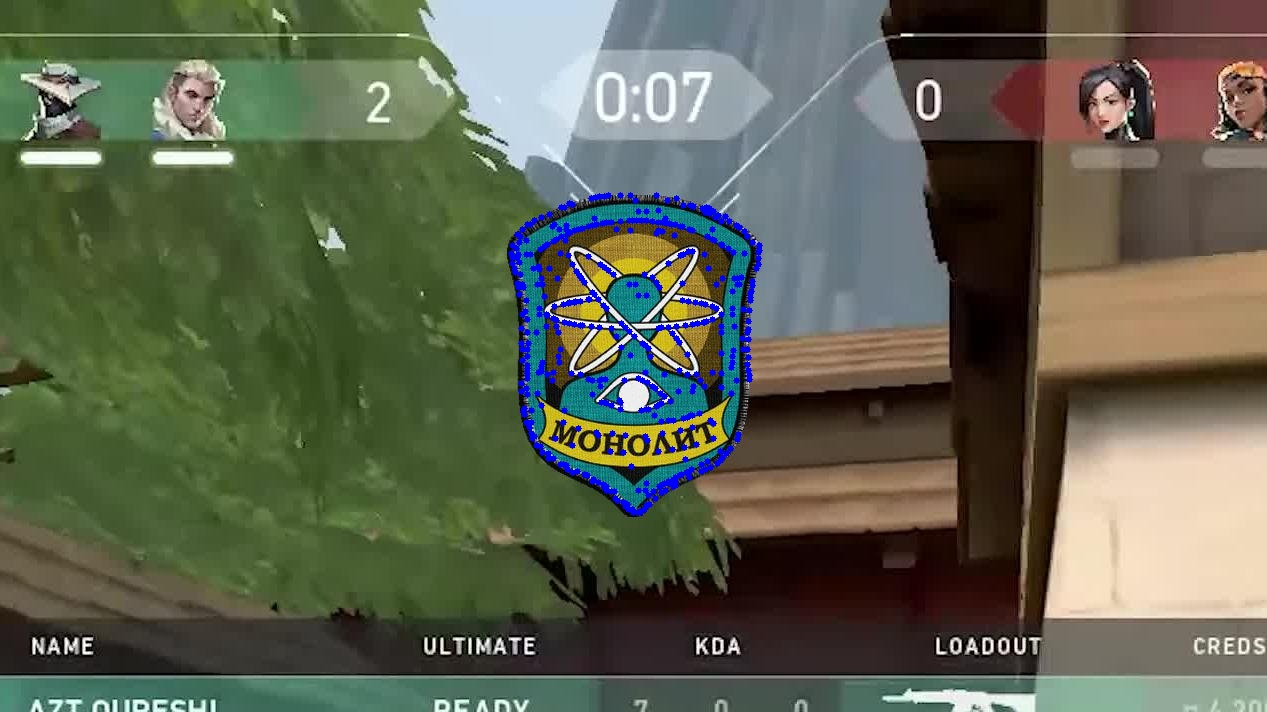
\includegraphics[width=0.8\textwidth]{ressources/image1_keypoints_masked.jpg}
    \caption{Overview of filtering process.}
    \label{fig:teacher_student}
\end{figure}
By repeating this process on both \textbf{reference} and \textbf{target} images, we get a pair of keypoint arrays ready to match using ALIKE's matching algorithm to finally get our training data samples.

\begin{figure}[H]
    \centering
    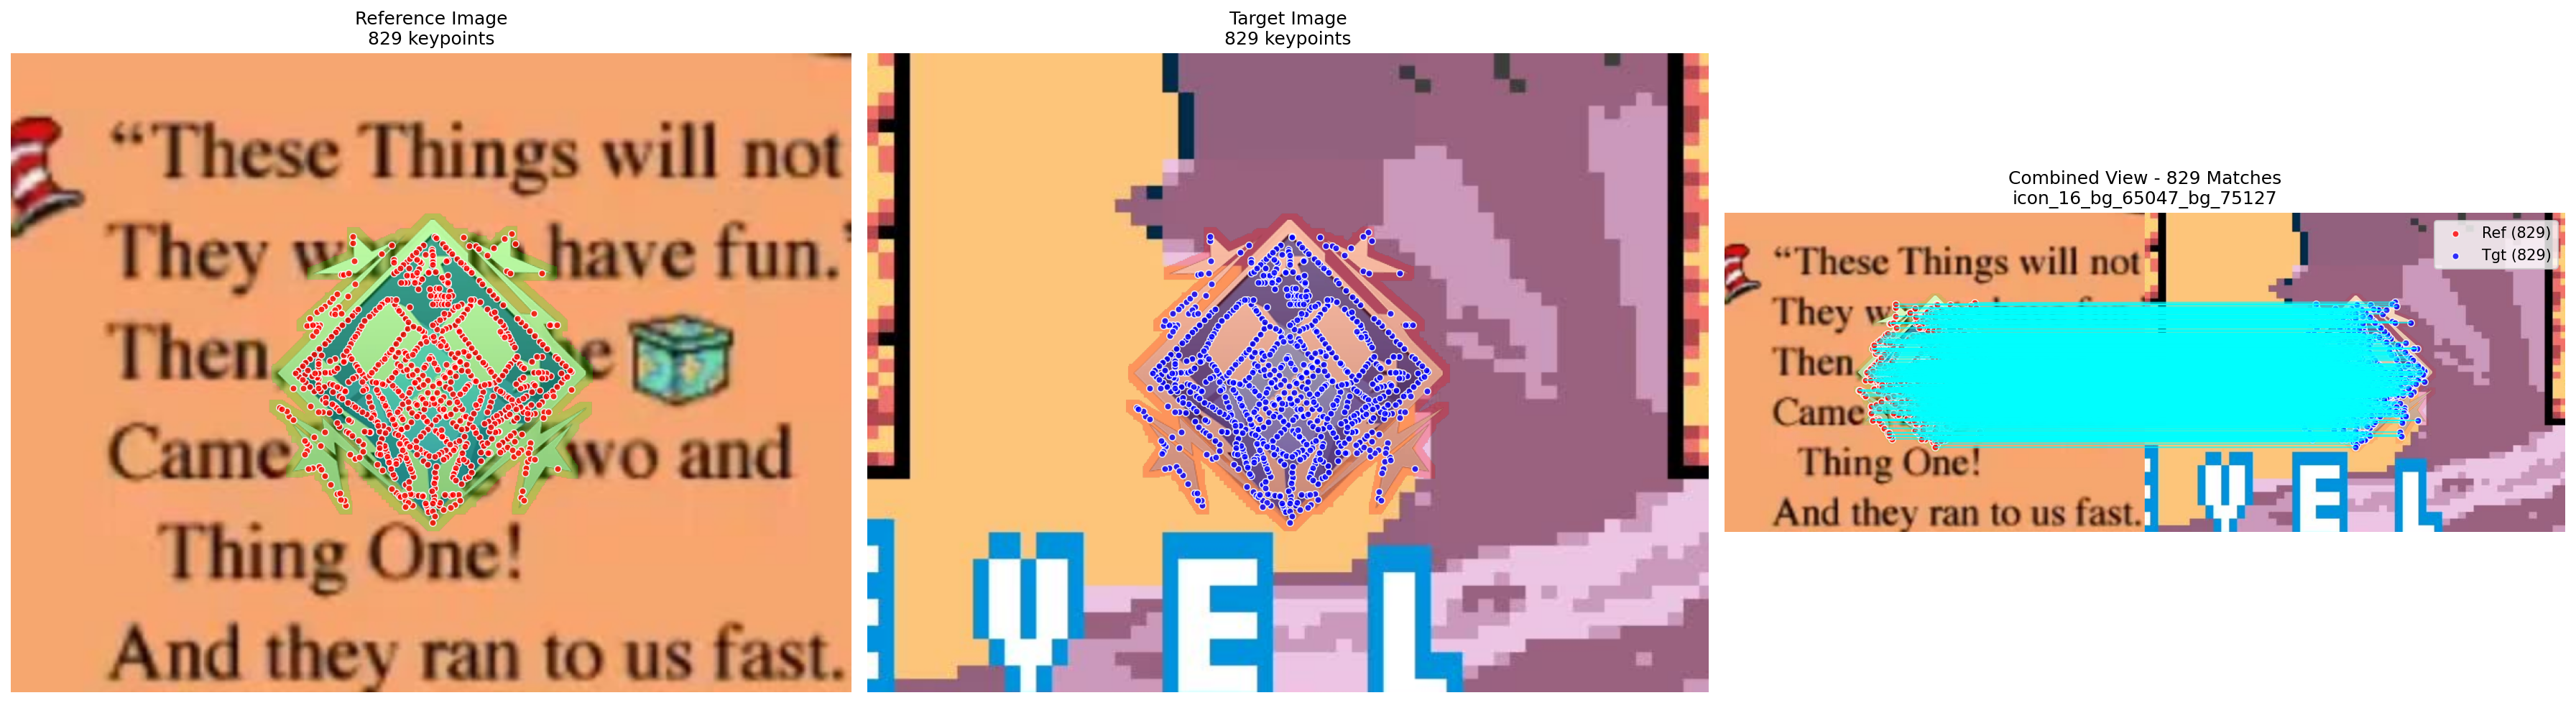
\includegraphics[width=\textwidth]{ressources/example_data1.png}
    \caption{Example of the synthesis process, showing the background and the overlaid icon as well as the detected keypoints and masks.}
    \label{fig:synthesis_example1}
\end{figure}
At a first time we trained the model following the default parameters:
\begin{itemize}
    \item Learning rate: 0.001
    \item Batch size: 10
    \item Number of iterations: 160k
\end{itemize}
This has led us to under average results, prompting further investigation into hyperparameter tuning and data formulation.
\subsection{Results}
The metrics obtained from our initial training runs indicate that while the
model is capable of learning the basic features of the icons, it struggles with
more complex backgrounds and variations in icon appearance.
\begin{figure}[H]
    \centering
    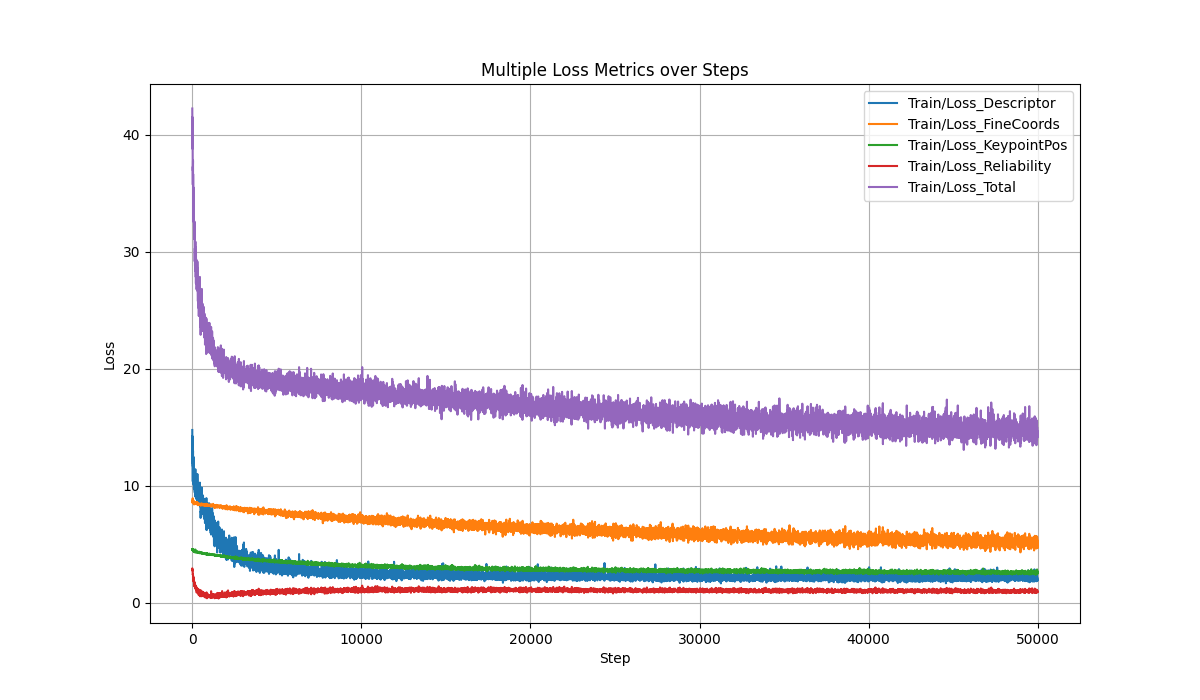
\includegraphics[width=\textwidth]{ressources/loss_1.png}
    \caption{Loss curves for initial training runs.}
    \label{fig:loss_curves_1}
\end{figure}
\begin{figure}[H]
    \centering
    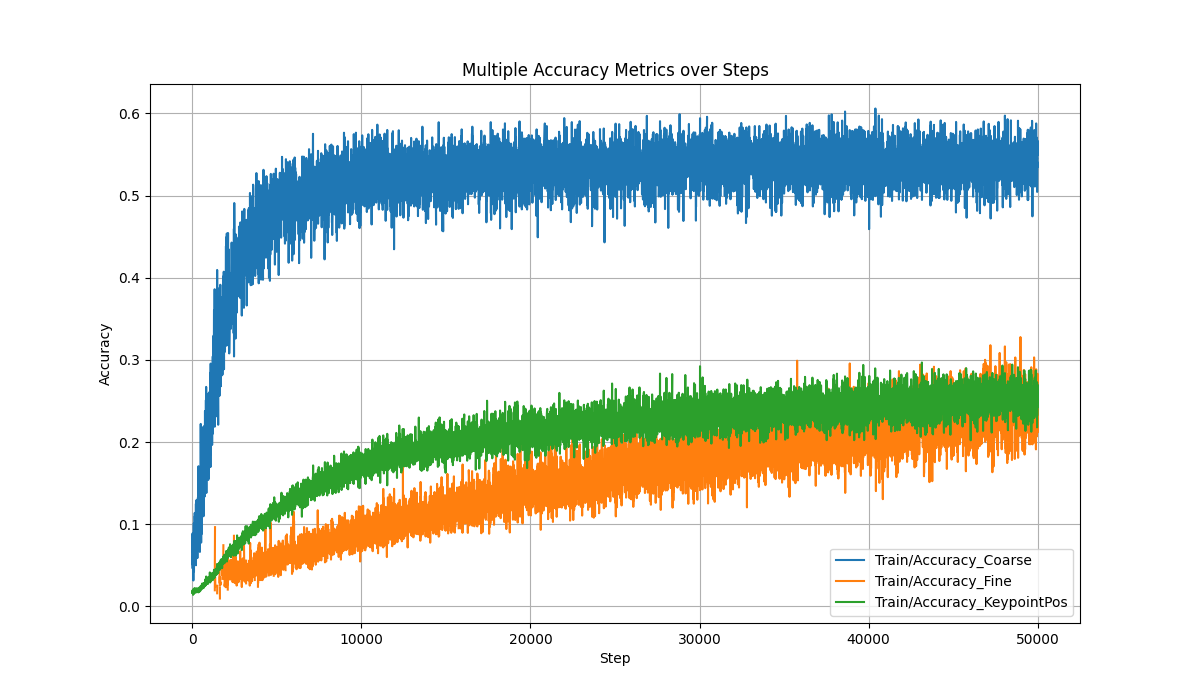
\includegraphics[width=\textwidth]{ressources/acc_1.png}
    \caption{Accuracy curves for initial training runs.}
    \label{fig:acc_curves_1}
\end{figure}
\subsubsection{Accuracy Metrics}
\begin{itemize}
    \item \textcolor{blue}{\textbf{Coarse Accuracy: }}Rapid increase in the first ~5k steps, reaching ~55\%-60\%. Then it plateaus with small oscillations.
    \item \textcolor{darkgreen}{\textbf{Keypoint Position Accuracy: }}Steady growth until ~20k steps, then saturates around ~25\%-27\%.
    \item \textcolor{myorange}{\textbf{Fine Matching Accuracy: }}Slow but consistent improvement, reaching ~20\%-22\% by step 50k, with more variance in later steps.
\end{itemize}
We can interpret this as follows:
\begin{itemize}
    \item The model learns coarse correspondences very quickly and maintains that
          performance, suggesting early layers or coarse matching blocks converge fast.
    \item Fine matching is the slowest to improve, likely because it depends on the
          coarse stage being strong first, and needs more subtle feature learning.
    \item Keypoint position accuracy plateaus mid-training, meaning spatial localization
          stops improving after ~20k steps.
\end{itemize}
\subsubsection{Loss Metrics}
\begin{itemize}
    \item \textcolor{blue}{\textbf{Descriptor Loss: }}Sharp drop in the first $\sim$5k steps, then remains low and stable (around 1--2).
    \item \textcolor{myorange}{\textbf{Fine Coordinates Loss: }}Slow but steady decrease across the 50k steps, still trending down by the end of training.
    \item \textcolor{darkgreen}{\textbf{Keypoint Position Loss: }}Drops quickly in early training and stabilizes, mirroring the accuracy plateau.
    \item \textcolor{red}{\textbf{Reliability Loss: }}Low from the start with minimal change, indicating stable confidence estimation.
    \item \textcolor{purple}{\textbf{Total Loss: }}Large drop in the first $\sim$5k steps, followed by a slower but continuous decline until the end.
\end{itemize}

We can interpret this as follows:
\begin{itemize}
    \item Most of the learning happens in the first 5k--10k steps, especially for
          descriptors and keypoint positioning.
    \item Fine coordinate refinement remains the main bottleneck, as its loss is still
          higher and accuracy is still improving, suggesting more training could help.
    \item Reliability loss stability shows that confidence estimation remains consistent
          throughout training.
\end{itemize}

\subsubsection{Confusion matrix}
\begin{figure}[H]
    \centering
    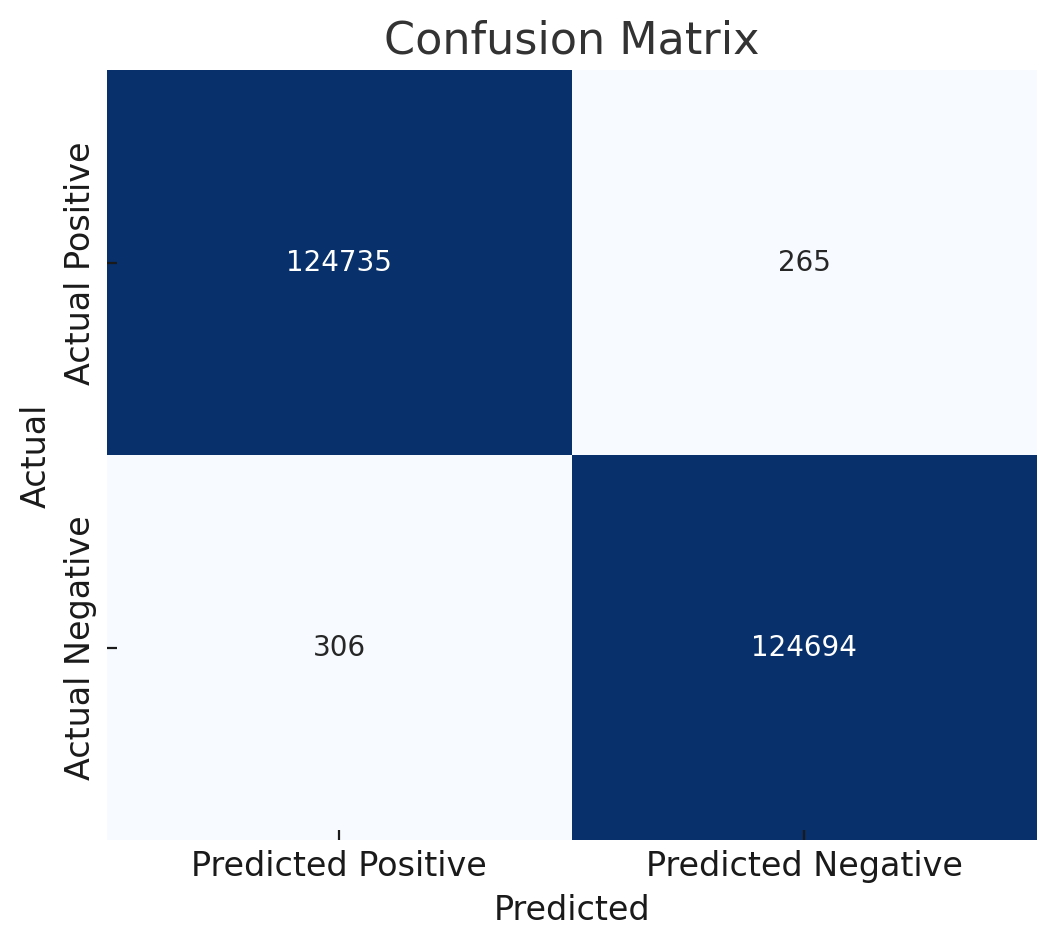
\includegraphics[width=0.7\textwidth]{ressources/confusion_matrix_1.png}
    \caption{Confusion matrix for initial training runs.}
    \label{fig:confusion_matrix_1}
\end{figure}
The confusion matrix shows the following values:
\begin{itemize}
    \item \textbf{True Positives (TP):} 124,735 cases where positive samples were correctly classified.
    \item \textbf{False Negatives (FN):} 265 cases where positive samples were incorrectly classified as negative.
    \item \textbf{False Positives (FP):} 306 cases where negative samples were incorrectly classified as positive.
    \item \textbf{True Negatives (TN):} 124,694 cases where negative samples were correctly classified.
\end{itemize}

From these values, we can compute:
\begin{itemize}
    \item \textbf{Accuracy:} $\frac{TP + TN}{TP + TN + FP + FN} \approx 99.77\%$
    \item \textbf{Precision:} $\frac{TP}{TP + FP} \approx 99.76\%$
    \item \textbf{Recall:} $\frac{TP}{TP + FN} \approx 99.79\%$
    \item \textbf{F1-Score:} $\approx 99.78\%$
\end{itemize}

These results indicate that the model performs extremely well, with both
precision and recall above 99.7\%, suggesting minimal misclassification in both
classes, but not enough, as False positives are extremely important in our
case, as they would lead to false matches, and ultimately impact the user
experience negatively.
\subsubsection{Overall Assessment}
The training shows strong performance in terms of fast convergence on coarse
matching and descriptor learning, with stable behavior and no signs of
divergence. However, fine matching accuracy remains low compared to coarse
accuracy, and keypoint accuracy saturates early, indicating possible
underfitting in fine localization. \textbf{To address these issues, several
    strategies can be considered: extending the training or applying fine-tuning
    with a smaller learning rate to further improve fine accuracy, reweighting the
    losses to give more emphasis to the FineCoords component once the coarse stage
    has converged, and applying data augmentation techniques that highlight
    sub-pixel differences to strengthen fine matching capabilities. Additionally, a
    curriculum learning approach could be adopted, starting with simpler examples
    before progressively increasing difficulty for the fine stage. }

\section{Iterative Refinement}
During experimentation, we implemented and evaluated three alternative
synthesis pipelines derived from our general concept:
\begin{enumerate}
    \item \textbf{NAFM A – Static Background-Icon, Transformed Keypoints:}
          The background and icons remained unchanged, while the keypoints were transformed using the homography matrix generated during the synthesis process. This matrix was applied to map the keypoints from the reference image to the target image, rather than re-extracting them from both images using the teacher model.
    \item \textbf{NAFM B – Cropped Background/Dynamic Icon-Transformed Keypoints:}
          The reference image was cropped down to focus on the area of interest, and ignore the background. The target icon was transformed using translation, placing it in a random position within the background.
    \item \textbf{NAFM C – Unfiltered SIFT Features}
          The reference and target images were not changed from the variant B, but the keypoints were extracted and matched using SIFT, without filtering them using the binary mask.
\end{enumerate}
Each variant maintained the core pipeline (ROI selection, overlay, keypoint extraction, matching), but emphasized different aspects of visual variability.
\subsection{Variant A}
In variant A, we focused on maintaining a static background and icon, while
transforming the keypoints obtained from the reference image to the target
image using a homography matrix. This would allow us to generate high quality
matches, as our objective is to find absolute correspondences between the
reference and the query templates. So we thought that using the transformed
keypoints would yield better results than re-extracting them from the target
image.
\subsubsection{Homography-based keypoint transfer}

Let the reference keypoints be $\mathcal{X}=\{ \mathbf{x}_i \}_{i=1}^{N}$ with
$\mathbf{x}_i=(u_i,v_i)^\top$ in pixel coordinates. Write them in homogeneous
form $\tilde{\mathbf{x}}_i=(u_i,v_i,1)^\top$. Let the homography be
$H\in\mathbb{R}^{3\times 3}$.

The mapped keypoints on the target image are
\[
    \tilde{\mathbf{x}}'_i \sim H\,\tilde{\mathbf{x}}_i,
    \qquad
    \mathbf{x}'_i=\Big(\frac{\tilde{u}'_i}{\tilde{w}'_i},\,
    \frac{\tilde{v}'_i}{\tilde{w}'_i}\Big)^\top,
\]
where $\tilde{\mathbf{x}}'_i=(\tilde{u}'_i,\tilde{v}'_i,\tilde{w}'_i)^\top$. In
matrix form for all points:
\[
    \tilde{X}' \sim H \tilde{X}, \quad
    X'=\begin{bmatrix}
        \tilde{X}'_{1,:}/\tilde{X}'_{3,:} \\[2pt]
        \tilde{X}'_{2,:}/\tilde{X}'_{3,:}
    \end{bmatrix}^{\!\top}.
\]

\paragraph{Notes.}
If $\tilde{w}'_i=0$ the point maps to infinity and is discarded.

\begin{figure}[H]
    \centering
    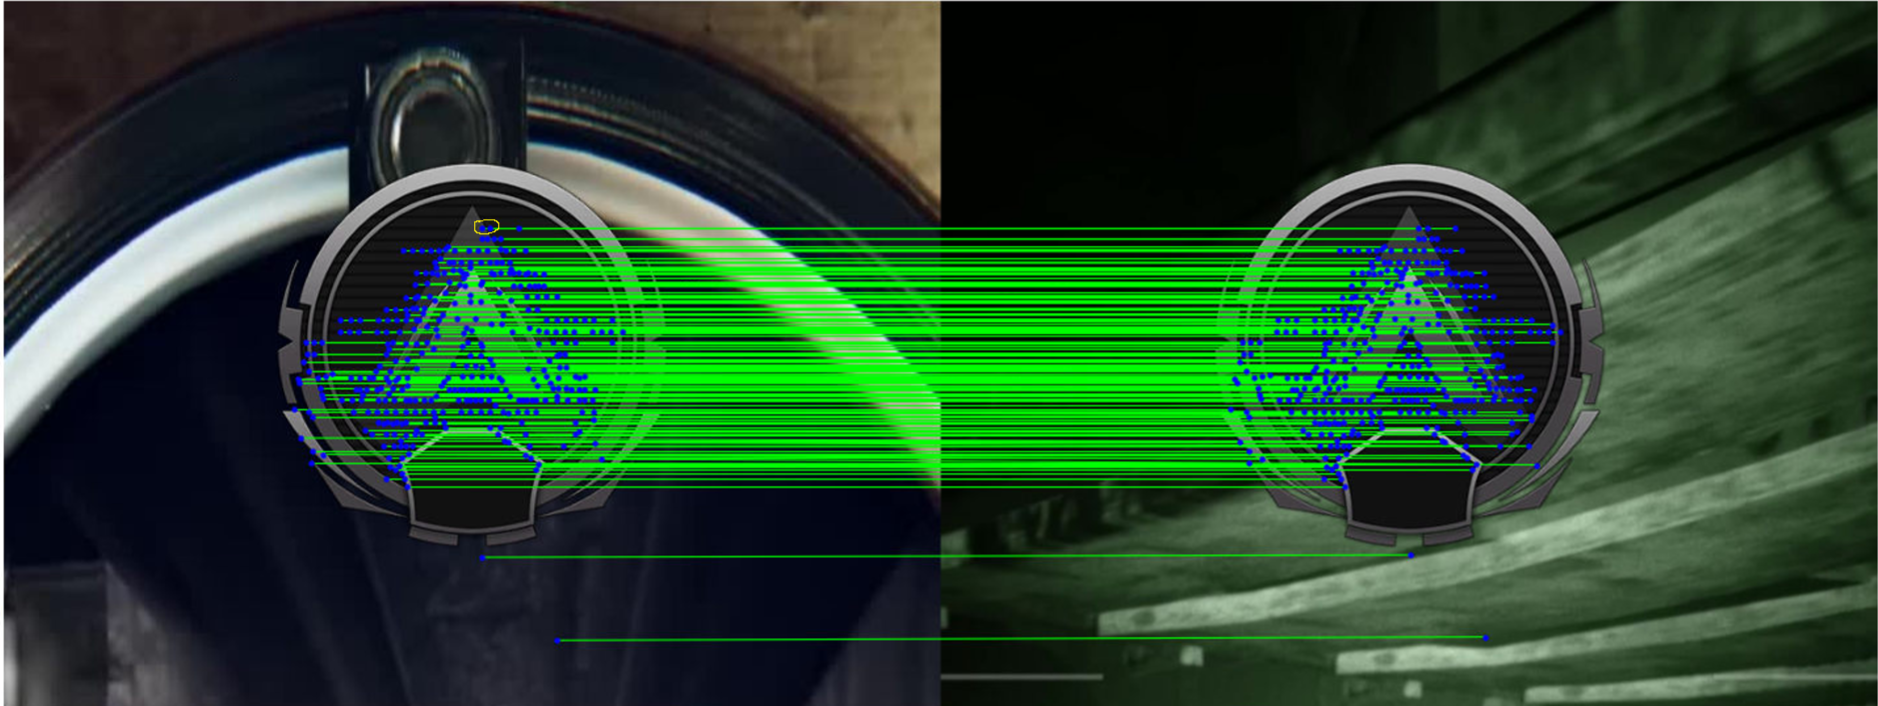
\includegraphics[width=0.6\textwidth]{ressources/image2.png}
    \caption{Example of the synthesis process for variant A}
    \label{fig:variant_a}
\end{figure}

Although this approach seems promising, it relies heavily on the quality of our
data synthesis process, and the homography matrix generation. In practice, we
found that the performance was sensitive to these factors.
\subsubsection{Accuracy metrics}
\begin{figure}[H]
    \centering
    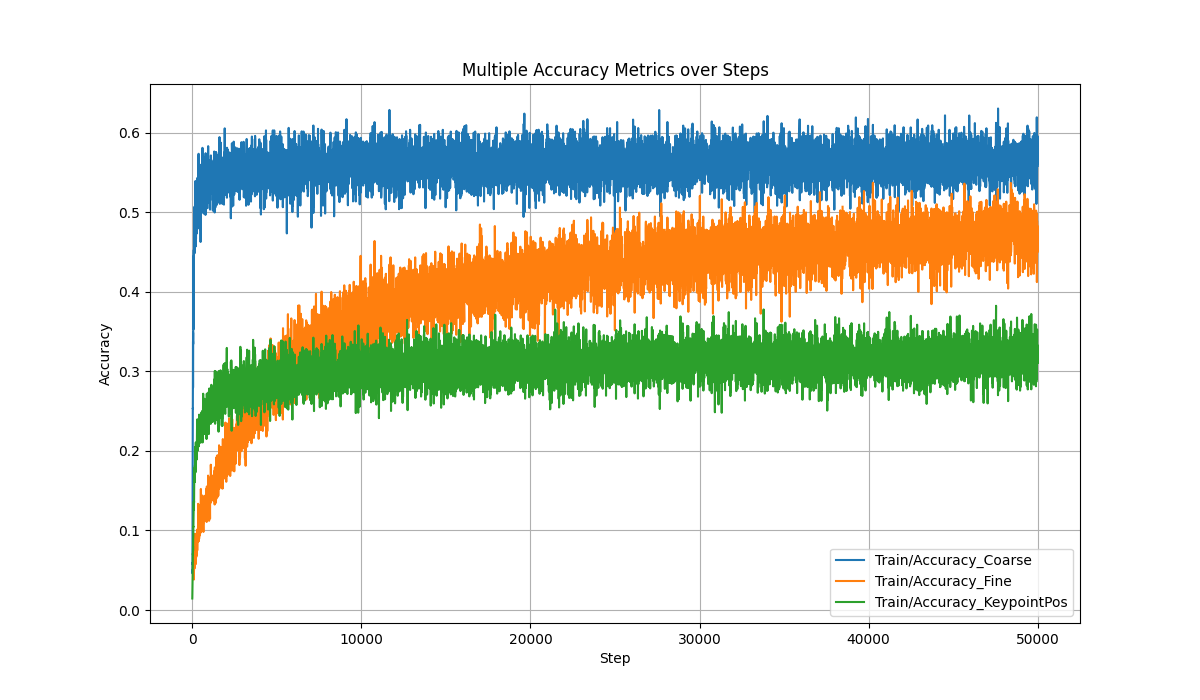
\includegraphics[width=0.7\textwidth]{ressources/acuracy_2.png}
    \caption{Example of the accuracy metrics evaluation}
    \label{fig:accuracy_metrics_2}
\end{figure}
\begin{itemize}
    \item \textcolor{blue}{\textbf{Coarse Accuracy: }}Starts low (~55\%) and quickly stabilizes around 60\%. Stable without large oscillations — suggests the coarse-level model component converged early.
    \item \textcolor{myorange}{\textbf{Fine Accuracy: }}Gradual increase from ~20\% to ~47\% over training — indicates steady improvement in fine-grained matching.
    \item \textcolor{darkgreen}{\textbf{Keypoint Position: }}Rises from ~10\% to ~36\%, slower than coarse accuracy, but still trending upward — likely due to higher difficulty of precise keypoint localization.
\end{itemize}
\subsubsection{Loss metrics}
\begin{figure}[H]
    \centering
    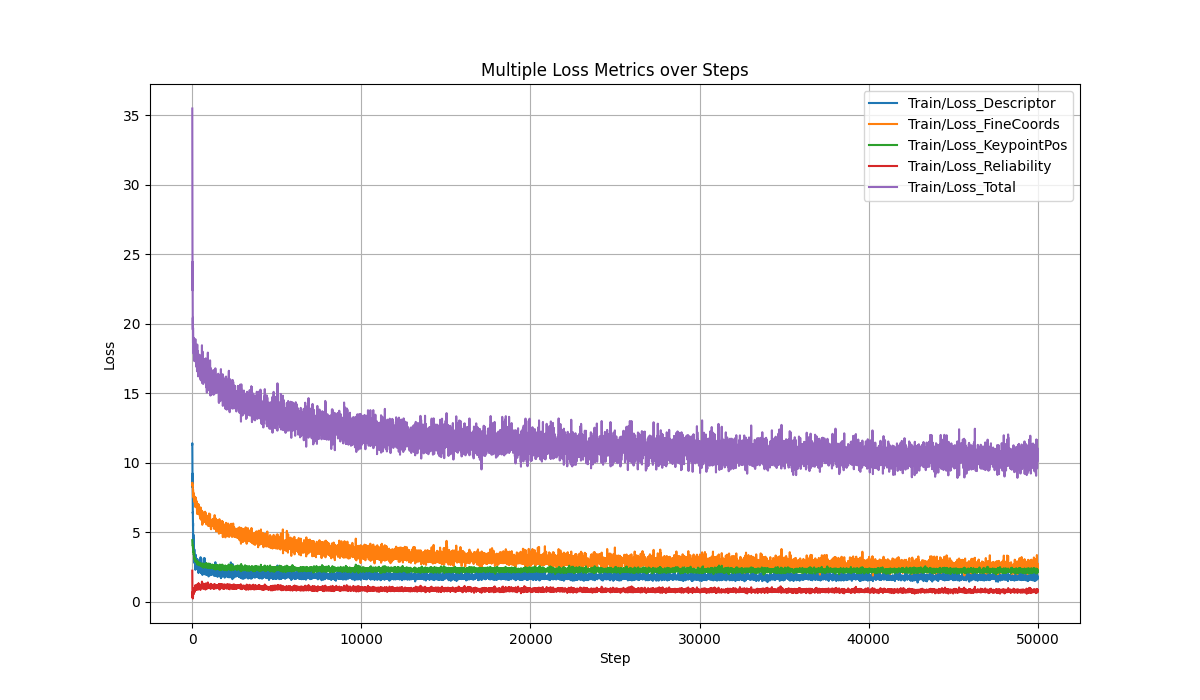
\includegraphics[width=0.7\textwidth]{ressources/multiple_losses_graph_2.png}
    \caption{Example of the loss metrics evaluation}
    \label{fig:loss_metrics_2}
\end{figure}
\begin{itemize}
    \item \textcolor{blue}{\textbf{Descriptor Loss:}} Rapid drop from ~17 to ~1.5 in the first 5k–10k steps, then slow decline — feature descriptors are learning quickly.
    \item \textcolor{myorange}{\textbf{Fine Coords Loss:}} Drops from ~8 to ~2.2, showing better coordinate regression.
    \item \textcolor{darkgreen}{\textbf{Keypoint Position Loss:}} Drops from ~4.5 to ~2.2 — still higher than fine coords, implying room for improvement in keypoint position accuracy.
    \item \textcolor{purple}{\textbf{Reliability Loss:}} Drops from ~2.5 to ~1.0 — confidence estimation is improving.
    \item \textcolor{red}{\textbf{Total Loss:}} Drops sharply from ~45 to ~12–14, then plateaus — convergence reached.
\end{itemize}
\subsubsection{Confusion Matrix}
\begin{figure}[H]
    \centering
    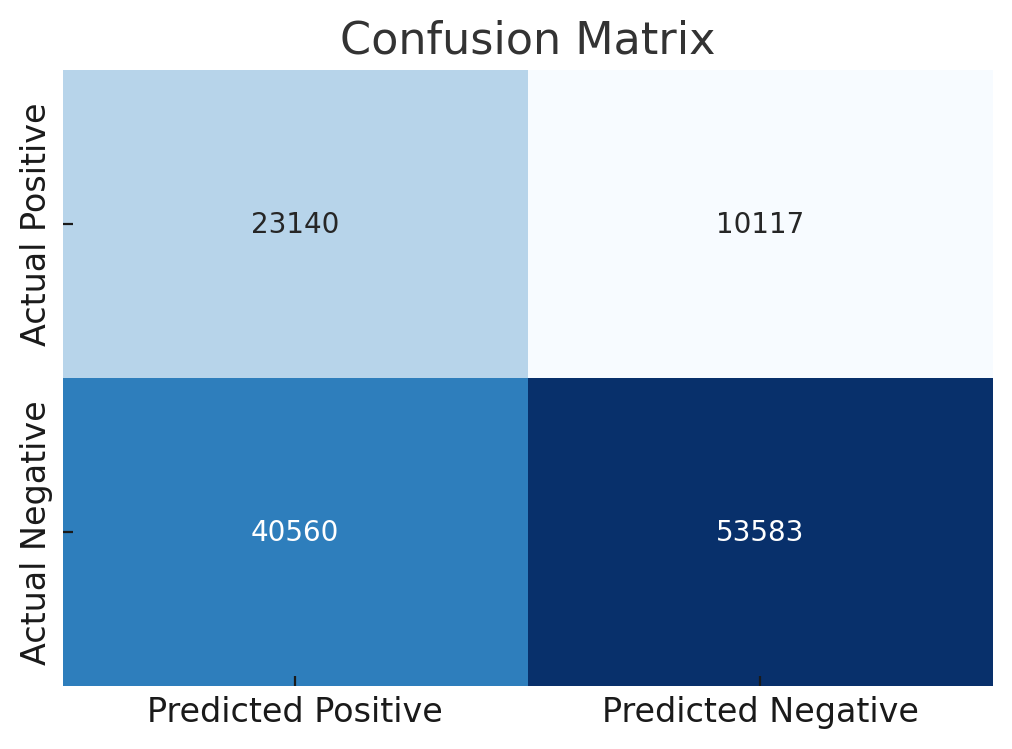
\includegraphics[width=0.6\textwidth]{ressources/confusion_matrix_2.png}
    \caption{Confusion matrix for variant A}
    \label{fig:confusion_matrix_2}
\end{figure}
\begin{itemize}
    \item \textbf{Accuracy :} 0.602
    \item \textbf{Precision :} 0.696
    \item \textbf{Recall :} 0.363
    \item \textbf{F1 Score :} 0.477
\end{itemize}
\subsubsection{Interpretation}
The results show that while the model can differentiate between various
features and capture some general patterns in the data, it struggles to truly
learn our custom target. The main problems are the rapid overfitting seen in
the loss curves and the overall low accuracy. To mitigate this, we introduced
learning rate scheduling and applied a basic form of data augmentation:
cropping the background from the reference image. This was done to prevent the
network from memorizing irrelevant background details instead of focusing on
the icon itself. Another issue was that the loss metrics operated on very
different scales, which could skew the optimization process. To address this,
we adjusted their relative weights so they would be more balanced. In
particular, we lowered the weight of the keypoint position loss, as it was
consistently the largest, to avoid it dominating the training signal. Despite
these changes, the network still fails to capture the distinctive patterns and
features that define our custom target.This suggests that the model is
focusing on general cues or noise rather than learning the precise visual
characteristics we aim to detect.
\begin{figure}[H]
    \centering
    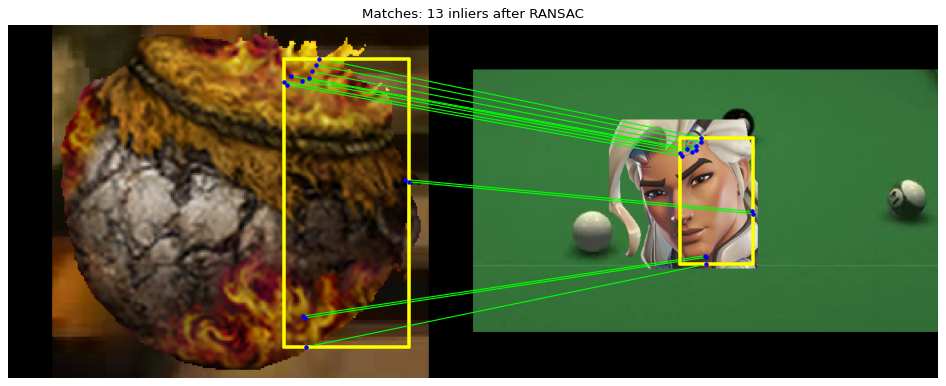
\includegraphics[width=0.7\textwidth]{ressources/false_positive_1.png}
    \caption{False Positive Example}
    \label{fig:false_positive_1}
\end{figure}

\subsection{Variant B}
In our new solution, we noticed that some icons contained semi-transparent
regions. When placed over a background, these pixels blended with the
background colors, creating a faint “merged” zone around and inside the icon.
This blending made the icon's edges less distinct and introduced background
information into what should be pure icon pixels. As a result, the network
could extract features from these shaded areas that are not native to the icon,
leading to confusing and noisy data and making it harder to learn accurate
features. To address this, we added a step in the data generation pipeline that
removes any pixel whose alpha value is below a chosen threshold, keeping only
fully opaque parts of the icon and ensuring a clean separation from the
background.
\begin{figure}[htbp]
    \centering
    \begin{minipage}{0.35\textwidth}
        \centering
        
\includegraphics[width=\textwidth]{ressources/icon_4_original.png}
        \caption{Original Icon}
        \label{fig:original_icon}
    \end{minipage}
    \hfill
    \begin{minipage}{0.35\textwidth}
        \centering
        
\includegraphics[width=\textwidth]{ressources/icon_4.png}
        \caption{Processed Icon}
        \label{fig:processed_icon}
    \end{minipage}
\end{figure}
Next we have added simple geometric transformations to our synthesis pipeline, where we would move the icon by random translations, to imitate the icon's position variability in real-world scenarios. And then we would keep the rest of the pipeline intact.
\begin{figure}[H]
    \centering
    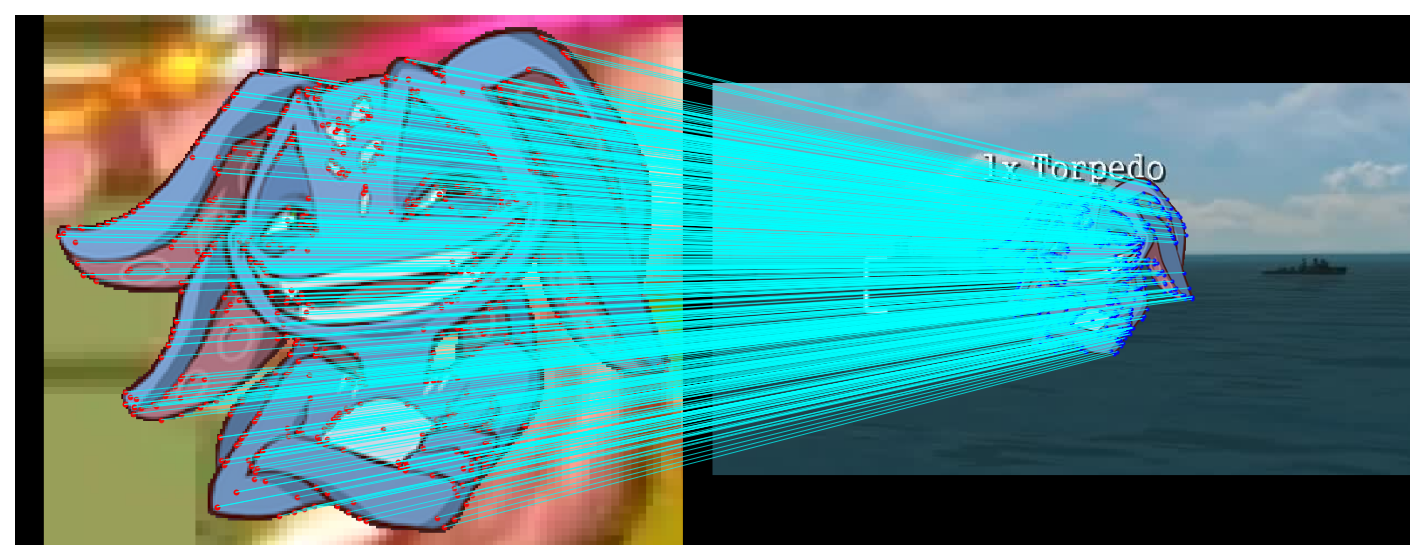
\includegraphics[width=0.8\textwidth]{ressources/image_3.png}
    \caption{Transformed Icon}
    \label{fig:transformed_icon}
\end{figure}
\subsubsection{Training Performance and Loss Analysis}

We conducted comprehensive training over 100,000 steps with multi-component
loss monitoring comprising coarse loss, fine loss, reliability loss, and total
loss, alongside validation evaluation every 1,000 steps. The training
demonstrated exceptional convergence across all metrics with a total loss
reduction of 78.1\% from 20.75 to 4.55.

\begin{figure}[H]
    \centering
    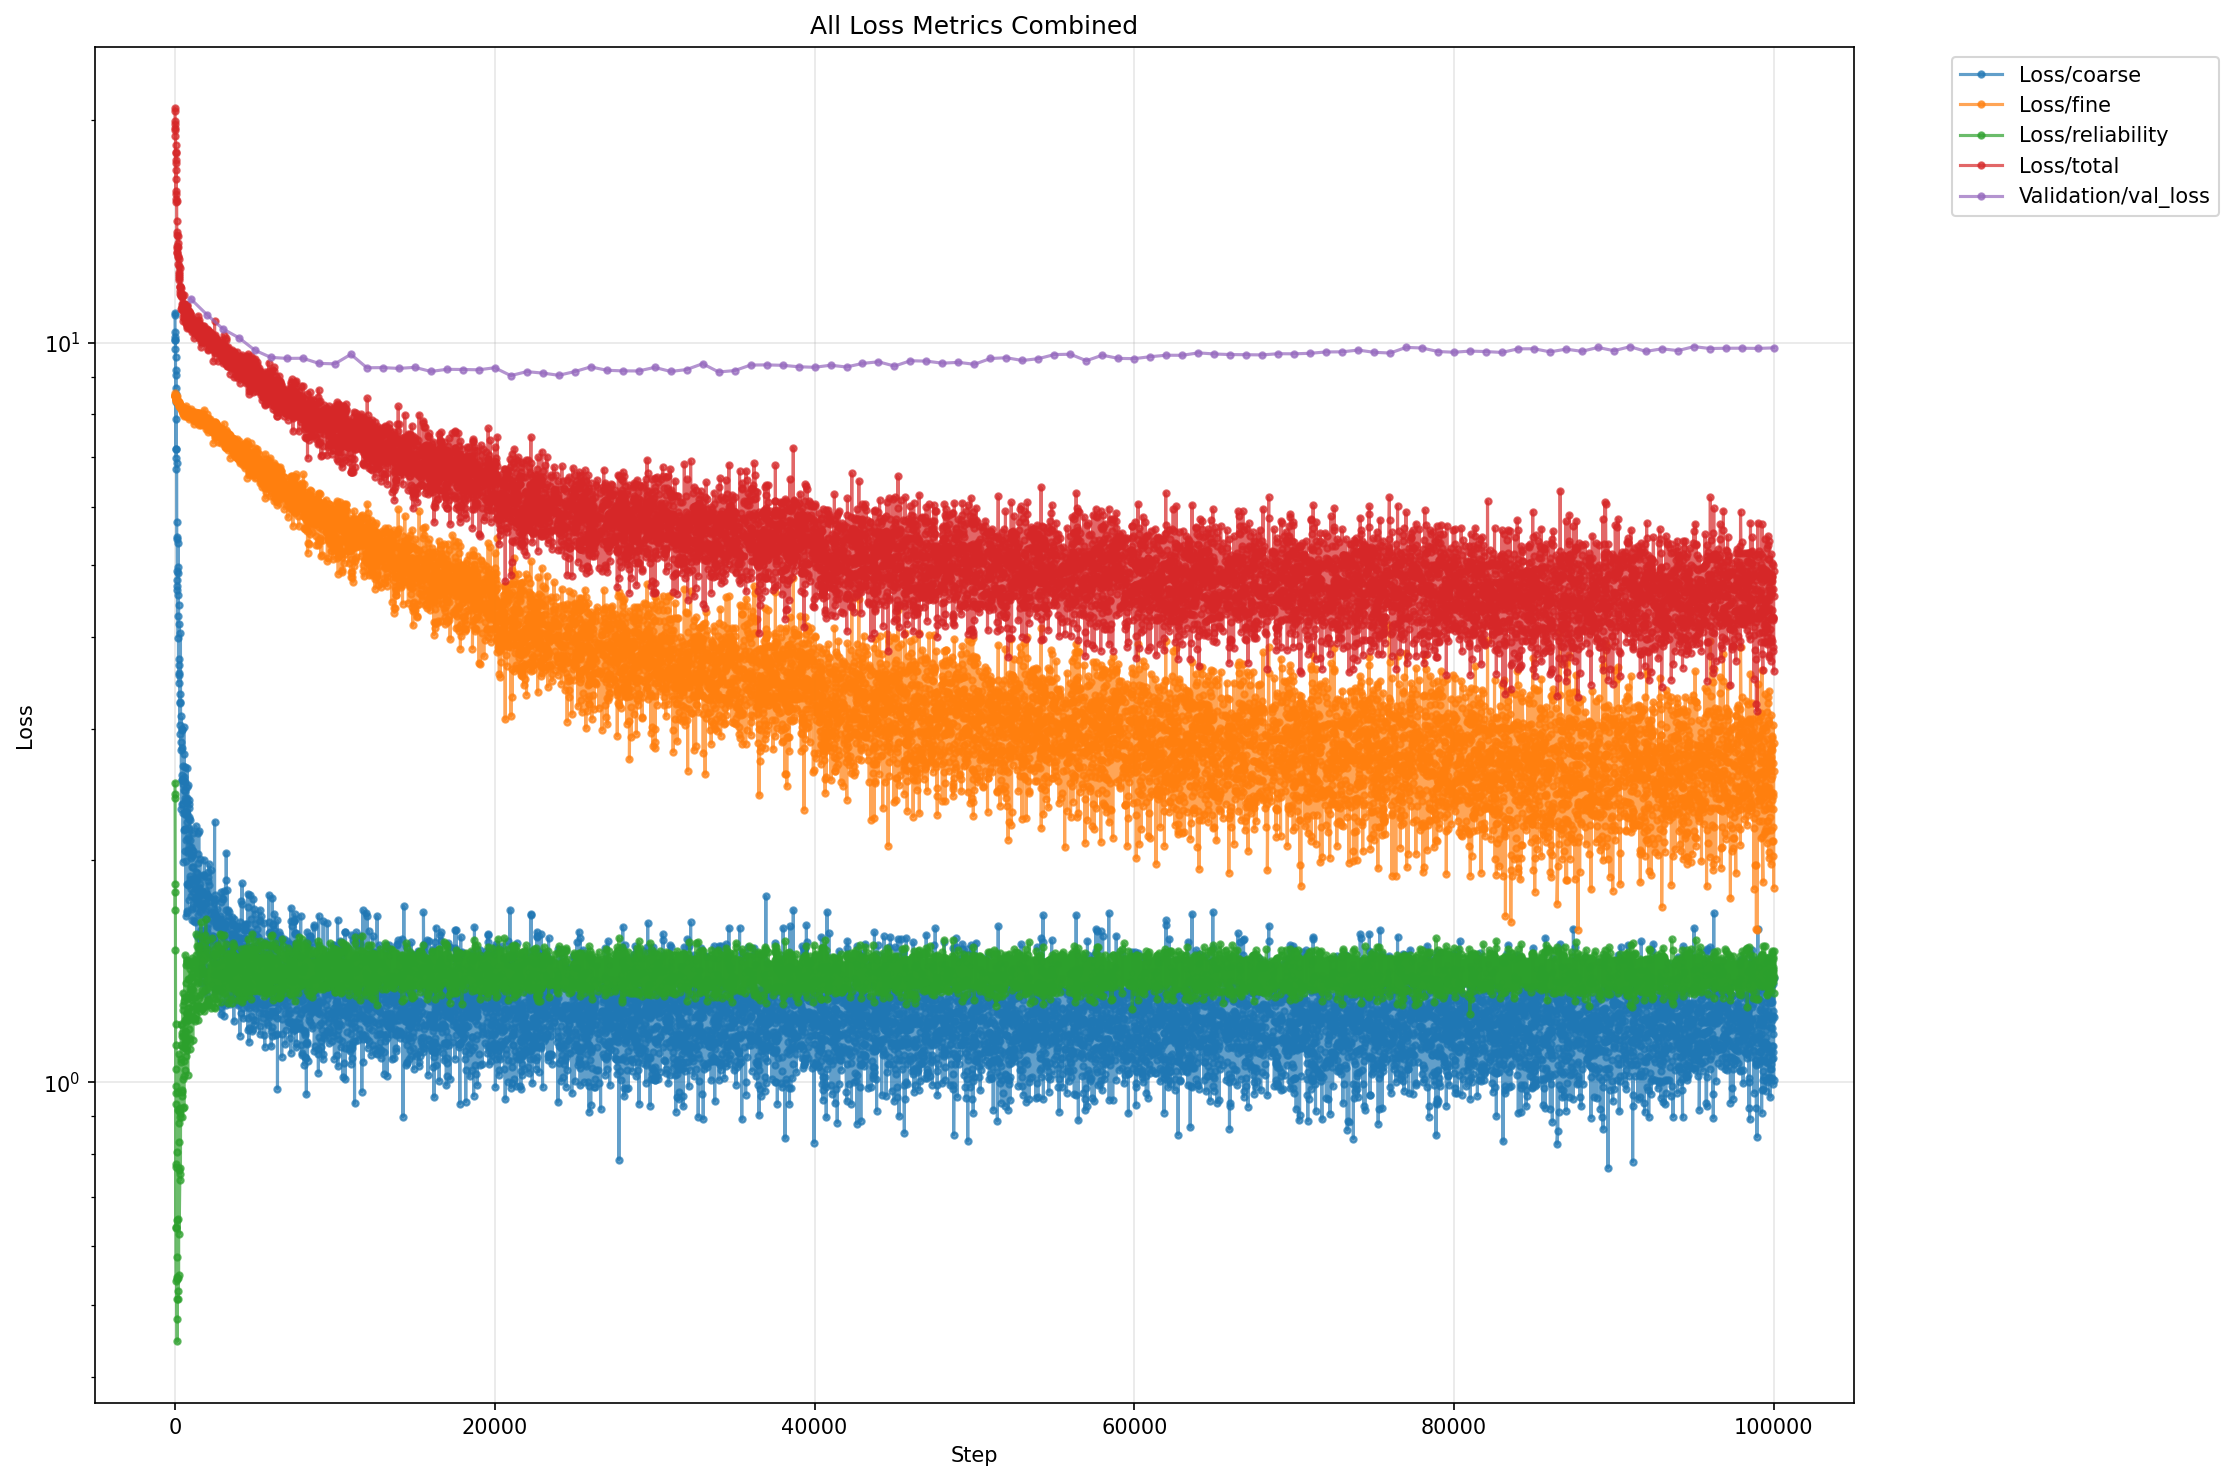
\includegraphics[width=0.8\textwidth]{ressources/loss_3.png}
    \caption{Loss Metrics}
    \label{fig:loss_components}
\end{figure}
The network exhibited rapid initial learning with total loss decreasing from 20.75 to approximately 8.0 within the first 20,000 steps. Component analysis revealed distinct optimization patterns: coarse loss achieved 88.8\% reduction (10.97→1.22), fine loss decreased by 69.1\% (8.51→2.63), and reliability loss improved by 45.4\% (2.54→1.39). This multi-faceted improvement indicates effective joint optimization across all network objectives (see Figure~\ref{fig:loss_components}).
\begin{figure}[H]
    \centering
    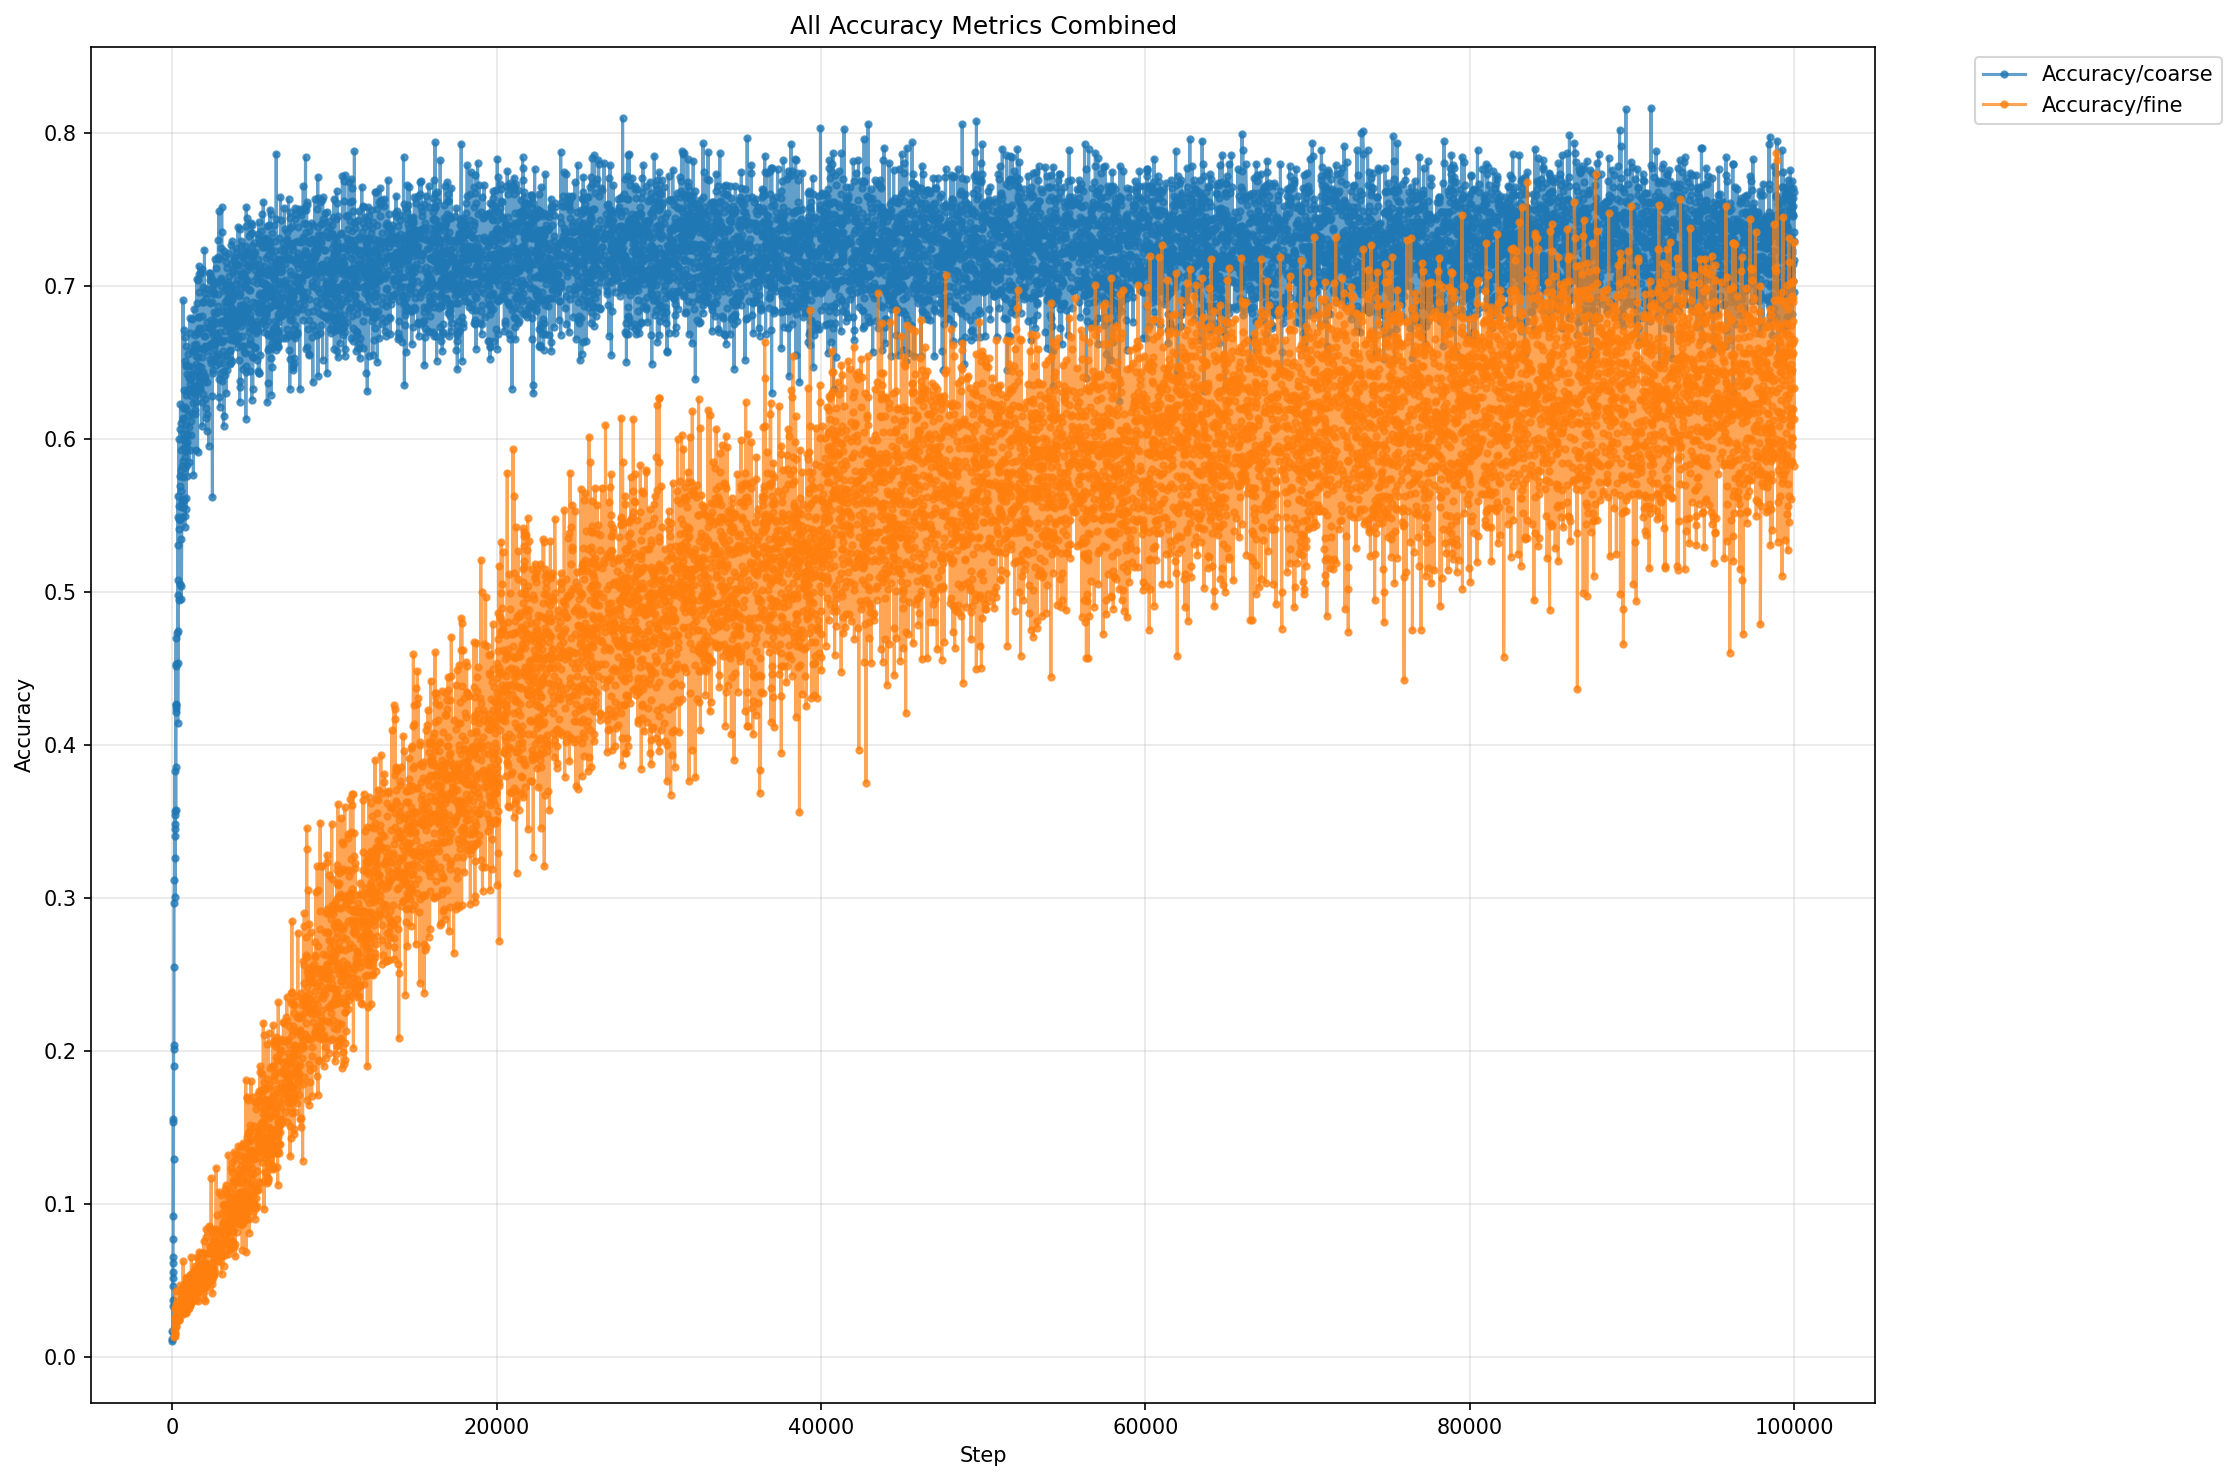
\includegraphics[width=0.8\textwidth]{ressources/accuracy_3.png}
    \caption{Accuracy Metrics}
    \label{fig:accuracy_metrics3}
\end{figure}

Accuracy metrics showed corresponding improvements, progressing from 1.01\% to
a peak of 81.65\% before stabilizing at 71.72\%. The validation loss trajectory
confirmed generalization capability, decreasing from 11.45 to 9.84 (14.1\%
improvement) with minimal overfitting indicators.
Figure~\ref{fig:accuracy_metrics3} illustrates the synchronized improvement
between accuracy and loss reduction throughout training.

The training exhibited three distinct phases: \textbf{rapid convergence} (0-20k
steps), \textbf{gradual refinement} (20k-70k steps), and \textbf{stabilization}
(70k-100k steps). All loss components demonstrated monotonic improvement with
minimal oscillations, indicating stable optimization dynamics. The final
validation loss of 9.84 and training accuracy of 71.72\% establish strong
baseline performance with excellent convergence properties.
\subsubsection{Confusion matrix}
\begin{figure}[H]
    \centering
    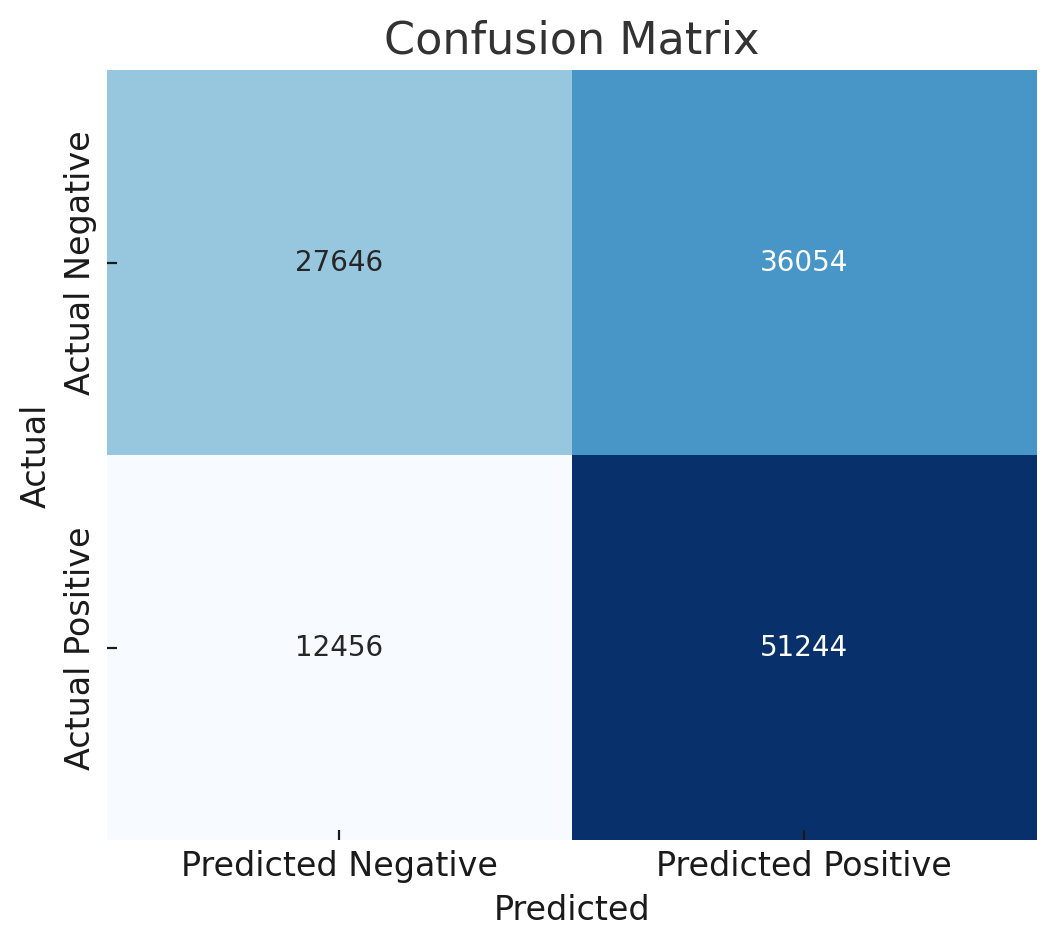
\includegraphics[width=0.7\textwidth]{ressources/confusion_matrix_3.png}
    \caption{Confusion matrix for variant B}
    \label{fig:confusion_matrix_3}
\end{figure}
\begin{itemize}
    \item \textbf{Accuracy: }0.619
    \item \textbf{Precision: }0.587
    \item \textbf{Recall: }0.804
    \item \textbf{F1 Score: }0.679
\end{itemize}
We could see that although the model can accurately detect the existence of keypoints, it still outputs an abnormally high false positive rate, which is a result of the overfitting of our model, and it not being able to generalize well to unseen data.
\subsubsection{Interpretation}
Although the training results show significant improvements in both loss and
accuracy metrics, the model still struggles with false positives, which is
result of the overfitting of our model. This could be proof that our choice of
teacher model is not optimal for this task, the low recall suggests the network learned to be overly conservative. This likely happened because of an insufficient number of negative examples. Perfect correspondences are great, but we also need to teach the network what NOT to match or that the model does not
generalize well to the target domain. To address this, we decided to explore an
alternative teacher model, and an alternative data formula.
\subsection{Variant C}
We decided to return to our original approach and adopt SIFT as the teacher
method. Given that our SIFT-based solution already demonstrates strong
performance on the target task, it provides a robust and reliable supervisory
signal for training. In addition, we deliberately removed all forms of
filtering, such as RANSAC and masking, in order to increase the complexity of
the learning problem and reduce the risk of overfitting. This choice results in
a more raw and unfiltered dataset, encouraging the student model to generalize
more effectively under challenging conditions. For the supervision of our
detector, we rely on SIFT to extract interest points from both the reference
and target images. Rather than using the associated descriptors, we retain only
the keypoint locations, which are sufficient for our purpose. These coordinates
are then converted into ground-truth heatmaps by encoding each keypoint as a
binary mask. Formally, let $\mathcal{K} = \{(x_i, y_i)\}_{i=1}^{N}$ denote the
set of detected keypoints in an image of size $H \times W$. The ground-truth
heatmap $M \in \{0,1\}^{H \times W}$ is defined as
\begin{equation}
    M(x,y) =
    \begin{cases}
        1, & \text{if } (x,y) \in \mathcal{K}, \\
        0, & \text{otherwise}.
    \end{cases}
\end{equation}
This representation allows us to jointly supervise both the detector and the descriptor using ground-truth correspondences between image pairs, following the training paradigm introduced in XFeat~\cite{xfeat2023}.

\begin{figure}[H]
    \centering
    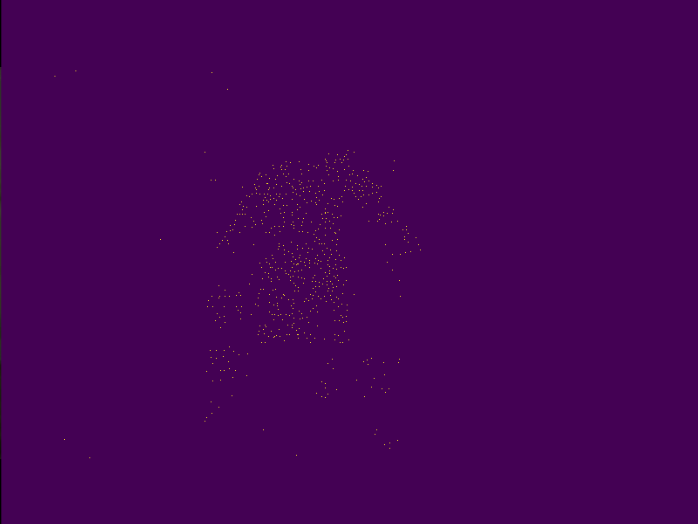
\includegraphics[width=0.8\textwidth]{ressources/image_41_heatmap.png}
    \caption{SIFT Keypoint Heatmap}
\end{figure}
Then we use These keypoints from both images to generate ground-truth correspondences.
\begin{figure}[H]
    \centering
    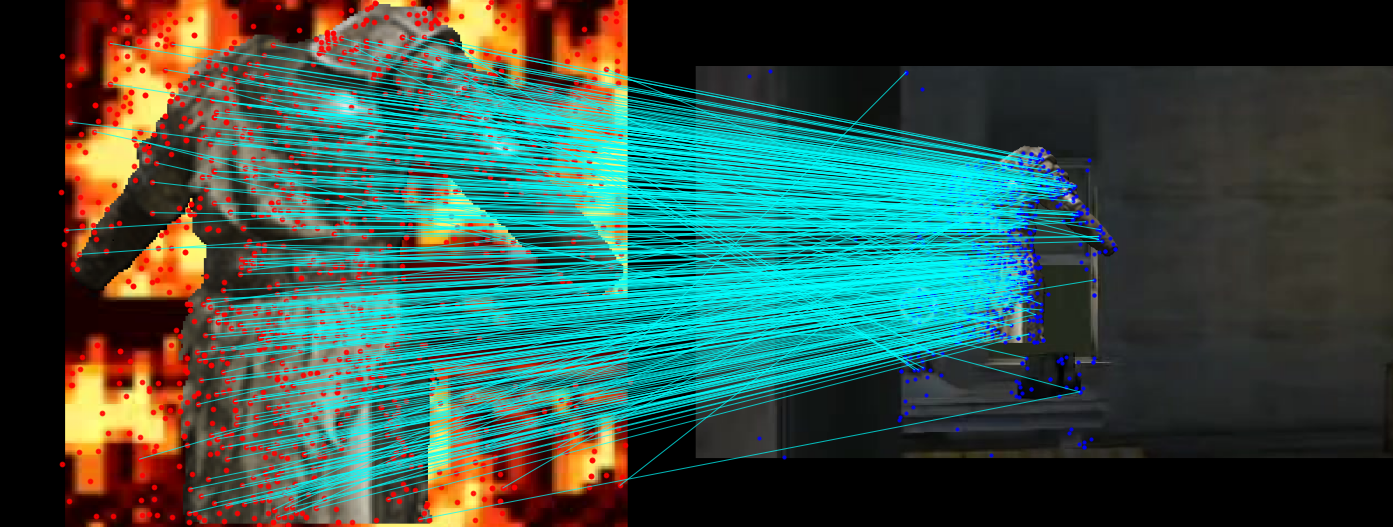
\includegraphics[width=0.8\textwidth]{ressources/image_41.png}
    \caption{SIFT Keypoint Detection Example}
    \label{fig:sift_example}
\end{figure}
\subsubsection{Training Performance and Loss Analysis}
We trained for \(\sim145\text{k}\) steps (0–144{,}688) with multi-component
loss monitoring (coarse, fine, reliability, and total) and validation every
1{,}000 steps. Optimization was decisive: the \textbf{total loss} fell by
\(\mathbf{81.65\%}\) from \(\mathbf{23.36}\rightarrow\mathbf{4.29}\), with a
rapid \(\mathbf{78.24\%}\) drop by \(\sim\)20k steps \((23.36\rightarrow
5.08)\). Component trends showed coordinated progress
(Fig.~\ref{fig:loss_components}): \textbf{coarse loss} improved
\(\mathbf{83.86\%}\) \((13.47\rightarrow 2.17)\), \textbf{fine loss}
\(\mathbf{81.51\%}\) \((8.64\rightarrow 1.60)\), and \textbf{reliability loss}
decreased more moderately by \(\mathbf{58.79\%}\) \((2.49\rightarrow 1.03)\).
Minima were reached early for reliability \((\mathbf{0.152}\ \text{at }
\mathbf{step\ 146})\) and coarse \((\mathbf{0.923}\ \text{at } \mathbf{step\
    6{,}276})\), with later troughs for fine \((\mathbf{1.003}\ \text{at }
\mathbf{step\ 129{,}639})\) and total \((\mathbf{3.718}\ \text{at }
\mathbf{step\ 129{,}639})\), consistent with a fast coarse/reliability
stabilization followed by slower fine-grained refinement.

\begin{figure}[H]
    \centering
    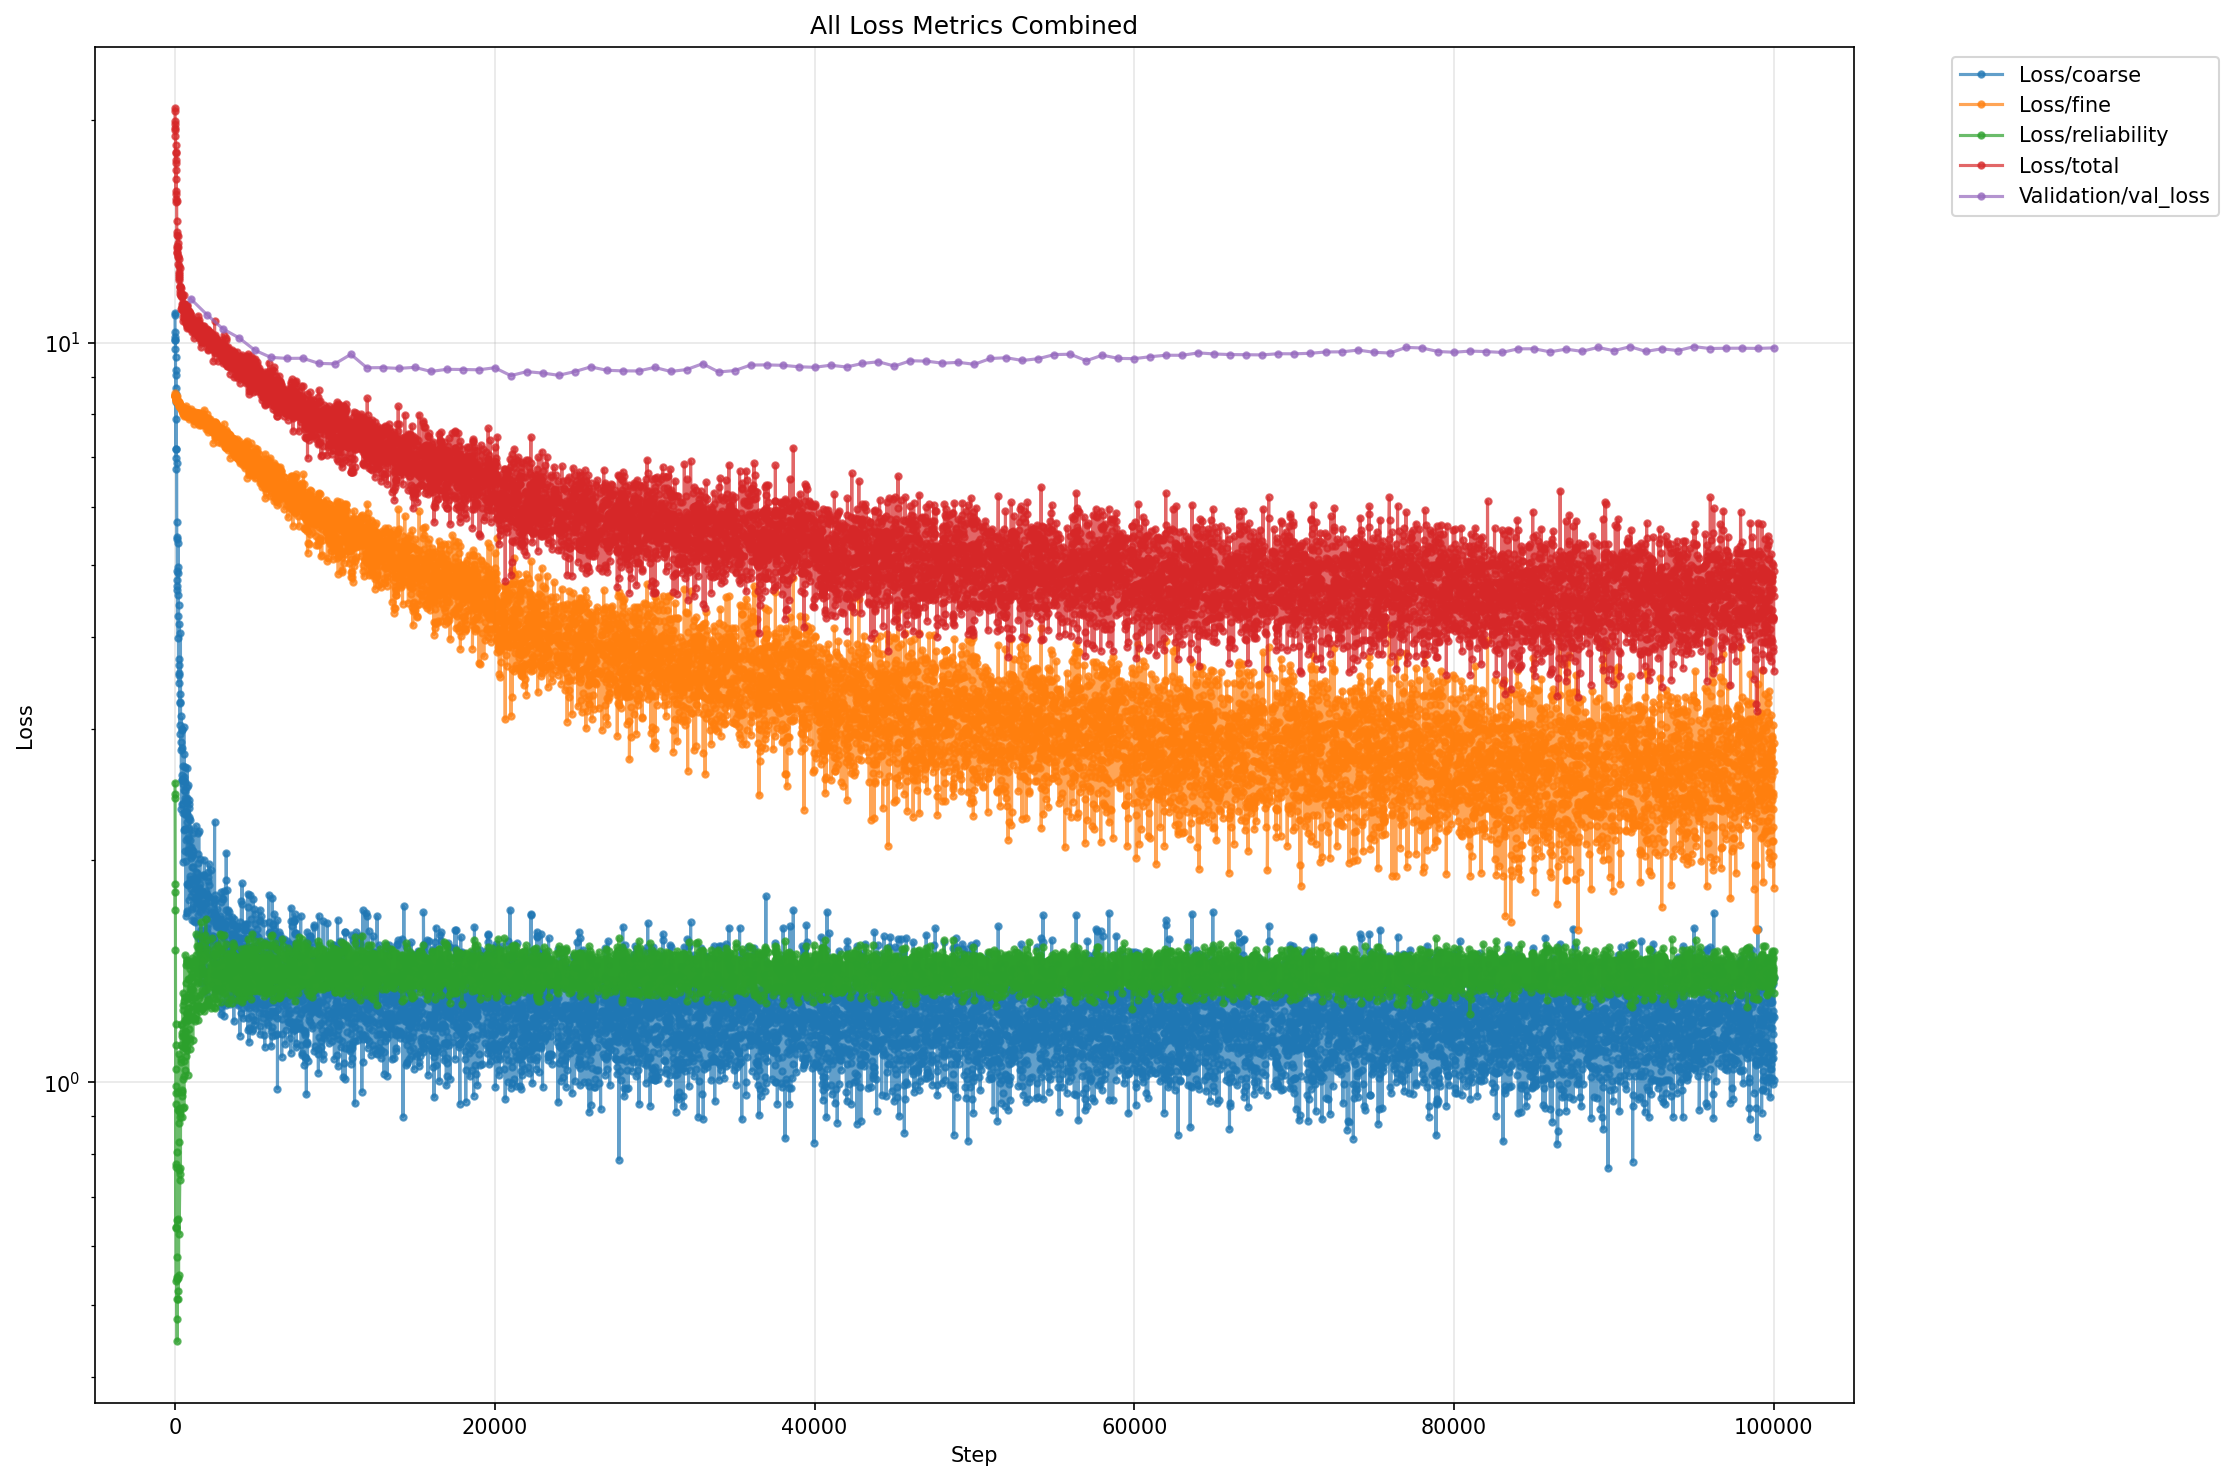
\includegraphics[width=0.8\textwidth]{ressources/loss_3.png}
    \caption{Loss Metrics}
    \label{fig:loss_components}
\end{figure}
Accuracy evolved in step with losses but with distinct behaviors across heads (Fig.~\ref{fig:accuracy_metrics3}). \textbf{Fine accuracy} peaked at \(\mathbf{100\%}\) (step \(\sim\)1{,}267) and stabilized at a strong late-training band (mean of last 10\% \(\approx \mathbf{78.62\%}\); final reading \(\mathbf{64.00\%}\)), indicating high-fidelity fine predictions despite endpoint variance. \textbf{Coarse accuracy} peaked at \(\mathbf{70.37\%}\) (step \(\sim\)63{,}515) but drifted downward thereafter (last-10\% mean \(\approx \mathbf{21.06\%}\); final \(\mathbf{15.14\%}\)), suggesting increasing sensitivity or over-confidence at the coarse stage as training progressed.

\begin{figure}[H]
    \centering
    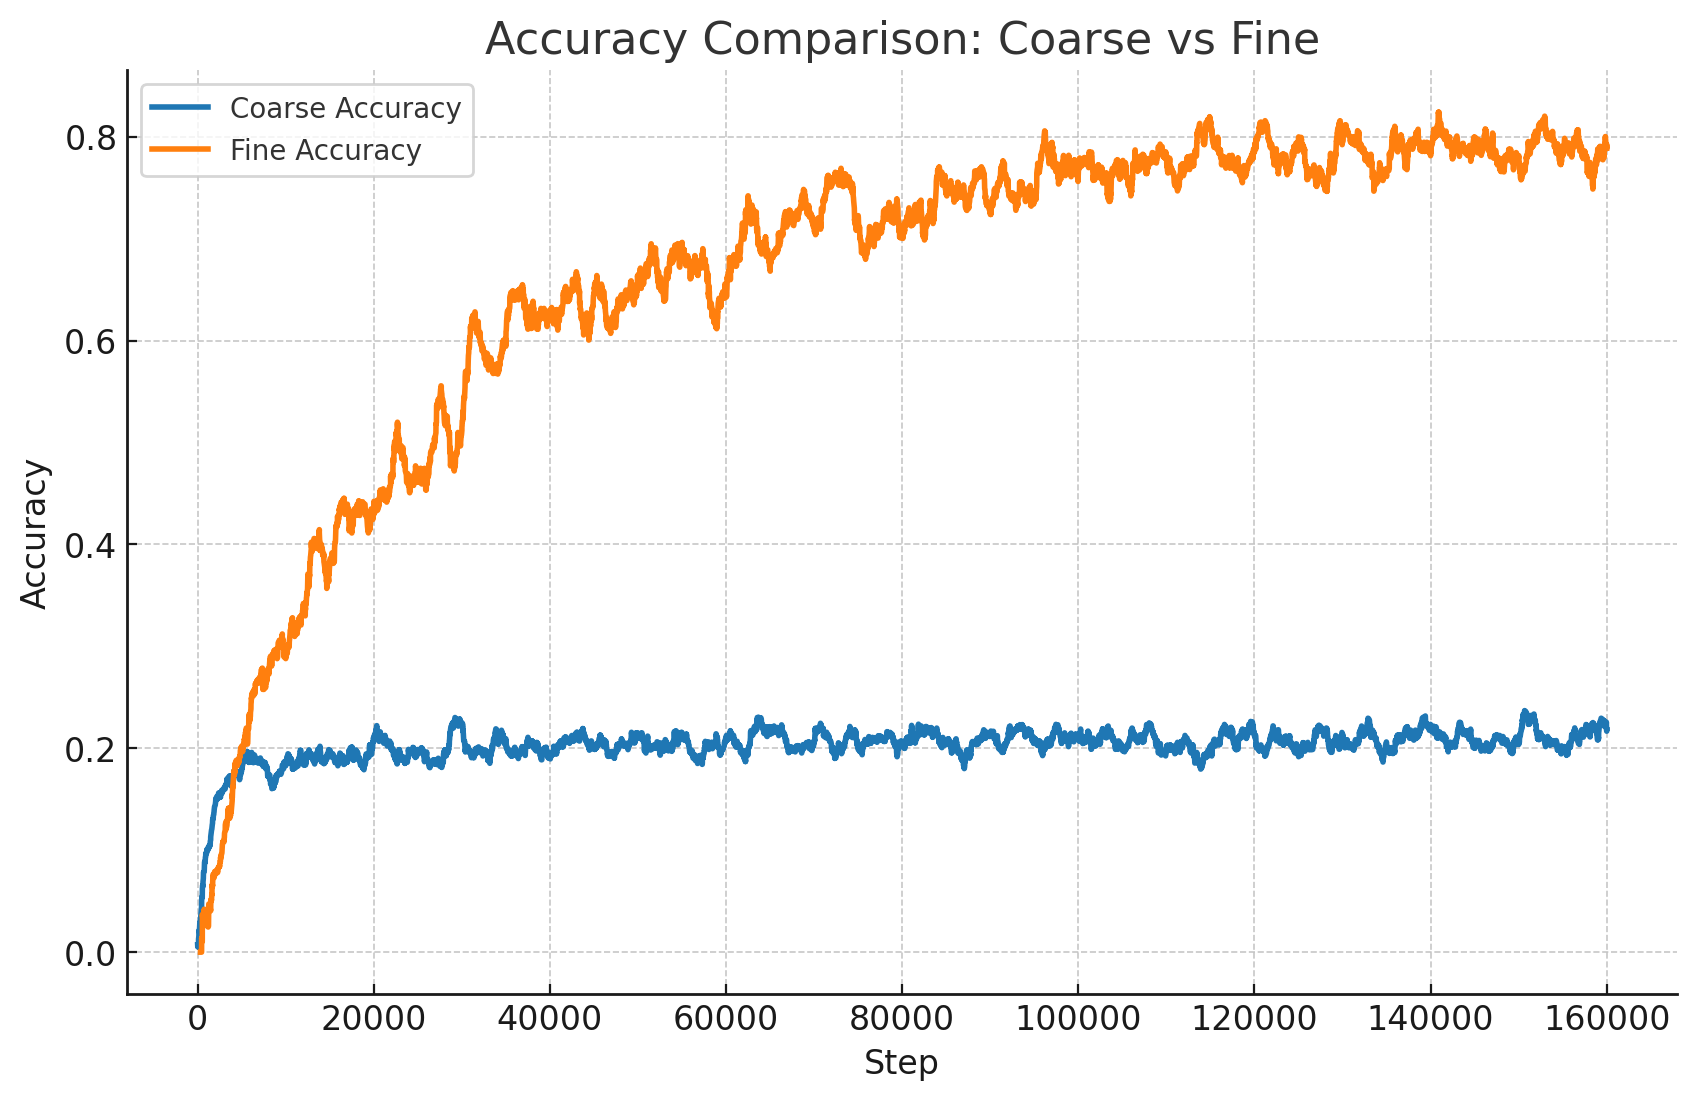
\includegraphics[width=0.8\textwidth]{ressources/accuracy_4.png}
    \caption{Accuracy Metrics}
    \label{fig:accuracy_metrics3}
\end{figure}

The validation trajectory clarifies generalization. It improved early
\((\mathbf{11.25}\ \text{at }999 \rightarrow \mathbf{10.20}\ \text{by
}\sim\!20\text{k}; \text{best } \mathbf{8.12}\ \text{at }\sim\!8\text{k})\),
then rose steadily to \(\mathbf{17.63}\) by the end, signaling late overfitting
despite continued training-loss gains. Overall, training exhibited three
phases: \textbf{rapid convergence} (0–20k), \textbf{gradual refinement}
(20k–100k), and a \textbf{late drift} (>100k) where optimization continues but
validation degrades. As a baseline, this run demonstrates excellent
optimization and mature fine-level accuracy; for deployment, prefer early
stopping around the validation minimum (\(\sim\)8–20k) or strengthen
regularization (e.g., heavier augmentation, dropout/weight decay, stochastic
depth) to preserve the early generalization peak while maintaining the gains in
fine accuracy.

\subsubsection{Confusion matrix}
\begin{figure}[H]
    \centering
    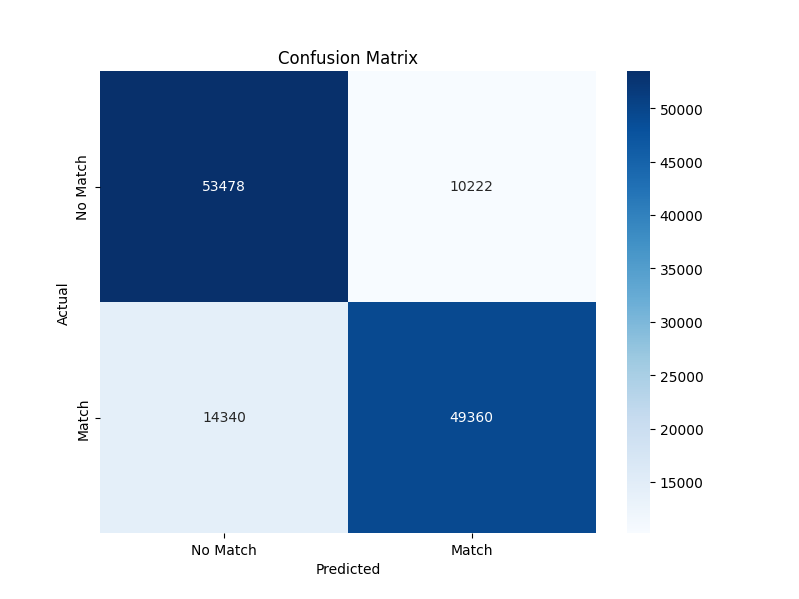
\includegraphics[width=0.8\textwidth]{ressources/cm_L_10.png}
    \caption{Confusion matrix for variant C}
    \label{fig:confusion_matrix_4}
\end{figure}
The new formula shows better promising results, the number of false positives has decreased significantly, increasing the overall precision of the model. With these results, this remains our best performing model so far, and we can see that the model is able to learn the keypoints and descriptors from the SIFT teacher model, and generalize well to unseen data.

